%% Type de document et encodage de la police
\documentclass[a4paper]{article}
\usepackage[utf8x]{inputenc}

%% Initialise la taille des pages et des marges
\usepackage[a4paper,top=3cm,bottom=3cm,left=2cm,right=2cm,marginparwidth=1.75cm]{geometry}

%% Packs utiles
\usepackage{amsmath}
\usepackage{graphicx}
\usepackage[colorinlistoftodos]{todonotes}
\usepackage[colorlinks=true, allcolors=black]{hyperref}
\usepackage{fourier-orns}
\usepackage{titlesec}
\usepackage{fancyhdr}
\usepackage{fancyvrb}
\usepackage{array}
\usepackage{enumerate}

%% Ajout d'un sous-titre
\usepackage{titling}
\newcommand{\subtitle}[1]{%
  \posttitle{%
    \par\end{center}
    \begin{center}\large#1\end{center}
    \vskip0.5em}%
}

%% Permet la double intégrale \oiint
\usepackage{ esint }

%% Packs utiles pour la manipulation d'image
\usepackage{wallpaper}
\usepackage{amsfonts}
\usepackage{amssymb}
\usepackage{eso-pic}
\usepackage{multicol}

%% \setlength
\setlength{\parindent}{0.5cm}

%% \thefootnote
\renewcommand{\thefootnote}{\*}
\pagestyle{fancy} 
\setcounter{tocdepth}{5}

%% \headrulewidth
\renewcommand{\headrulewidth}{1pt}
\fancyhead[C]{} 
\fancyhead[L]{}
\fancyhead[R]{\footnotesize{\leftmark}}

%% \footrulewidth
\renewcommand{\footrulewidth}{1pt}
\fancyfoot[C]{} 
\fancyhead[L]{}
\fancyfoot[R]{\thepage}

%% definecolor
\definecolor{Zgris}{rgb}{0.87,0.85,0.85}

%% Redéfinition de la colonne d'un tableau pour que ses éléments soient centrés sur l'axe vertical
%% Implique l'utilisation de \tabularnewline à la place de \\ pour terminer une ligne du tableau
\newcolumntype{M}[1]{>{\raggedright}m{#1}}

%% Pack Tikz pour les diagrammes
\usepackage{tikz}
\usetikzlibrary{shapes.geometric, arrows, shapes, shapes.multipart, decorations.pathmorphing, backgrounds, positioning, fit, petri}

%% Pack circuitikz pour les circuits électriques
\usepackage{circuitikz}





\title{Électricité et magnétisme}
\subtitle{Sythèse du cours \textquotedblleft Physics II: Electricity and Magnetism" du MIT}
\author{Grégoire Roumache}
\date{Juillet 2017}

\begin{document}

\maketitle

































\section{Loi de Coulomb}











\subsection{Théorie}





\begin{itemize}
    \item La force électrique exercée par une charge $ q_1 $ sur une seconde charge $ q_2 $ est donnée par la \textbf{loi de Coulomb}:
\[ \vec{\textbf{F}}_{12} = k_e \frac{q_1 q_2}{r^2} \hat{\textbf{r}} = \frac{1}{4 \pi \epsilon_0} \frac{q_1 q_2}{r^2} \hat{\textbf{r}} \]
où $\displaystyle k_e = \frac{1}{4 \pi \epsilon_0} = 8.99 \times 10^9 \; N \; m^2/C^2 \approx 9\times 10^9 $ est la constante de Coulomb.
    \item Le \textbf{champ électrique} en un point de l'espace est défini comme la force électrique agissant sur une charge test $ q_t $
divisée par $ q_t $: 
\[ \vec{\textbf{E}} = \frac{\vec{\textbf{F}}_e}{q_t} \]
    \item Le champ électrique à une distance $ r $ de la charge $ q $ vaut:
\[ \vec{\textbf{E}} = \frac{1}{4 \pi \epsilon_0} \frac{q}{r^2} \hat{\textbf{r}} \]
    \item Avec le \textbf{principe de superposition}, on détermine que le champ électrique dû à plusieurs charges, chacune ayant une 
charge $ q_i $ et se trouvant à une distance $ r_i $ est: 
\[ \vec{\textbf{E}} = \frac{1}{4 \pi \epsilon_0} \sum_i \frac{q_i}{r_i^2} \hat{\textbf{r}}_i \]
    \item Une particule de charge $ q $ et de masse $ m $ se déplaçant dans un champ électrique $ \vec{\textbf{E}} $ a une accélération: 
\[ \vec{\textbf{a}} = \frac{q \vec{\textbf{E}}}{m} \]
    \item Un \textbf{dipôle électrique} consiste en deux charges opposées (par exemple $ +q $ et $ -q $) séparées par une distance $2 a$.
Le moment dipolaire électrique (utile notamment en chimie: $ H_2 O $ est une molécule dipolaire) est représenté par un vecteur $ \vec{\textbf{p}} $ qui pointe de la charge négative vers la charge positive et possède une magnitude de: 
\[ p = 2 a q \]
    \item Le \textbf{moment de force} agissant sur un dipôle électrique dans un champ électrique extérieur uniforme est: 
\[ \vec{\boldsymbol{\tau}} = \vec{\textbf{p}} \wedge \vec{\textbf{E}} \]
    \item L'\textbf{énergie potentielle} d'un dipôle électrique dans un champ électrique extérieur uniforme est: 
\[ U = - \vec{\textbf{p}} \cdot \vec{\textbf{E}} \]
    \item Le champ électrique en un point de l'espace dû à une distribution continue de charge d'éléments de charge $ d q $ est: 
\[ d \vec{\textbf{E}} = \frac{1}{4 \pi \epsilon_0} \frac{d q}{r^2} \hat{\textbf{r}} \]
    \item Lorsque l'on s'étend loin assez d'une distribution de charge continue finie (pas de fil ou plan infini donc), l'expression analytique du champ électrique va ressembler à celui d'une charge ponctuelle.
\end{itemize}









\subsection{Pratique}






Comme expliqué dans la sous-section "Théorie", dans le cas d'une distribution continue de charge, on doit calculer l'intégrale vectorielle: \[ \vec{\textbf{E}} = \frac{1}{4 \pi \epsilon_0} \int \frac{d q}{r^2} \hat{\textbf{r}} \]
Pour réaliser l'intégration, on peut suivre la procédure suivante: 
\begin{enumerate}
    \item Commencer avec: $\displaystyle d \vec{\textbf{E}} = \frac{1}{4 \pi \epsilon_0} \frac{d q}{r^2} \hat{\textbf{r}} $
    \item Réécrire l'élément $ d q $ en: 
\[ d q =
\begin{cases}
\lambda \; d L      & \text{ (longueur) } \\
\sigma \; d A       & \text{ (aire) } \\
\rho \; d V         & \text{ (volume) }
\end{cases}
\]
selon la forme de distribution qui est soit en longueur, soit en surface, soit en volume.
    \item Remplacer $ d q $ dans l'expression de $ d \vec{\textbf{E}} $.
    \item Spécifier le système de coordonnées approprié (cartésien, cylindrique ou sphérique) et exprimer l'élément différentiel ($ d L, 
\; d A, \; d V $) ainsi que $ r $ en terme de coordonnées.

\begin{center}
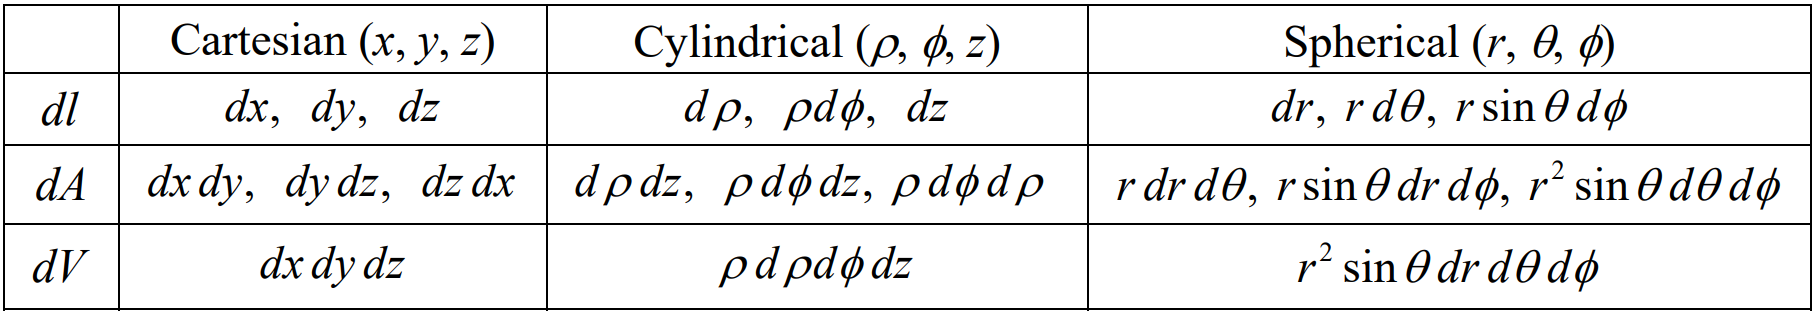
\includegraphics[width=0.8\textwidth]{coordonnees.PNG}
\end{center}

    \item Réécrire $ d \vec{\textbf{E}} $ en fonction des variables d'intégration et utiliser la symétrie pour identifier les composantes 
non-nulles du champ électrique.
    \item Compléter l'intégration pour obtenir $ \vec{\textbf{E}} $.
\end{enumerate}

\begin{center}
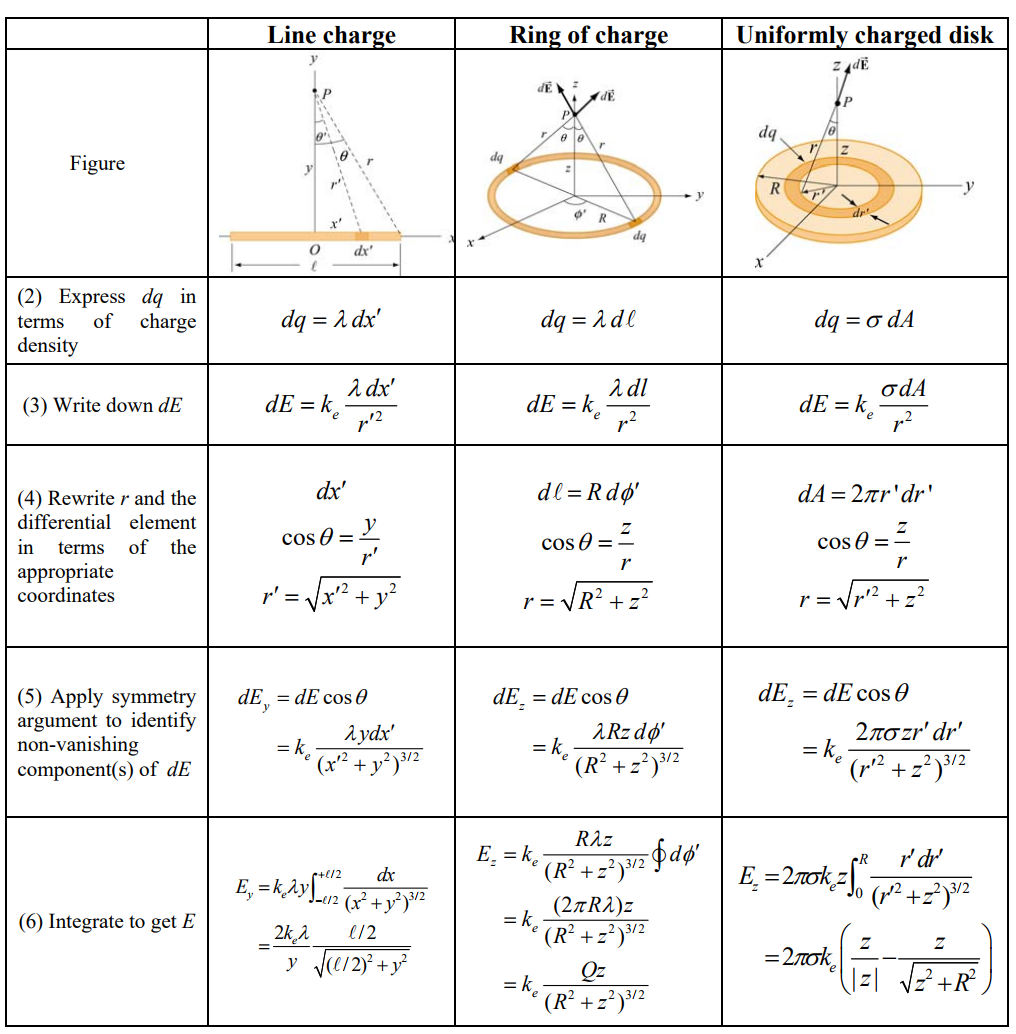
\includegraphics[width=\textwidth]{ExemplesFluxElec.PNG}
\end{center}






















\section{Potentiel électrique}











\subsection{Théorie}







\begin{itemize}
    \item Une force $ \vec{\textbf{F}} $ est \textbf{conservative} si l'intégrale curviligne sur une boucle fermée s'annule: 
\[ \oint \vec{\textbf{F}} \cdot d \vec{\textbf{s}} = 0 \]
    \item Le changement en énergie potentielle associé à une force conservative $ \vec{\textbf{F}} $ agissant sur un objet qui se déplace 
de $ A $ à $ B $ est: \[ \Delta U = U_B - U_A = - \int_A^B \vec{\textbf{F}} \cdot d \vec{\textbf{s}} \]
    \item La \textbf{différence de potentiel électrique} $ \Delta V $ entre les points $ A $ et $ B $ dans un champ électrique 
$ \vec{\textbf{E}} $ est donnée par: \[ \Delta V = V_B - V_A = \frac{\Delta U}{q_t} = - \int_A^B \vec{\textbf{E}} \cdot d \vec{\textbf{s}} \]
Cette grandeur représente la quantité de travail nécessaire pour déplacer une unité de charge du point $ A $ au point $ B $, sans changer son énergie cinétique.
    \item Le potentiel électrique d'une charge ponctuelle $ Q $ à une distance $ r $ vaut: 
\[ V = \frac{1}{4 \pi \epsilon_0} \frac{Q}{r} \]
Lorsqu'il y a plusieurs charges, on utilise le principe de superposition pour trouver le potentiel électrique: 
\[ V = \frac{1}{4 \pi \epsilon_0} \sum_i \frac{Q_i}{r_i} \]
    \item L'\textbf{énergie potentielle} associée à deux charges ponctuelles $ q_1 $ et $ q_2 $ séparées par une distance $ r_{12} $ est:
\[ U = \frac{1}{4 \pi \epsilon_0} \frac{q_1 q_2}{r_{12}} \]
    \item On peut, à partir du potentiel électrique $ V $, obtenir la valeur du champ électrique: 
\[ \vec{\textbf{E}} = - \nabla V \]
En coordonnées cartésiennes, les composantes peuvent être écrites de la manière suivante: 
\[ E_x = - \frac{\partial V}{\partial x}, \quad E_y = - \frac{\partial V}{\partial y}, \quad E_z = - \frac{\partial V}{\partial z} \]
    \item Le potentiel électrique dû à une distribution de charge continue est: 
\[ V = \frac{1}{4 \pi \epsilon_0} \int \frac{d q}{r} \]

\end{itemize}










\subsection{Pratique}







Comme expliqué dans la sous-section "Théorie", dans le cas d'une distribution continue de charge, on doit calculer l'intégrale vectorielle: \[ V = k_e \int \frac{d q}{r} \]
Pour réaliser l'intégration, on peut suivre la procédure suivante: 
\begin{enumerate}
    \item Commencer avec: $\displaystyle d V = \frac{1}{4 \pi \epsilon_0} \frac{d q}{r} $
    \item Réécrire l'élément $ d q $ en: 
\[ d q =
\begin{cases}
\lambda \; d L      & \text{ (longueur) } \\
\sigma \; d A       & \text{ (aire) } \\
\rho \; d V         & \text{ (volume) }
\end{cases}
\]
selon la forme de distribution qui est soit en longueur, soit en surface, soit en volume.
    \item Remplacer $ d q $ dans l'expression de $ d V $.
    \item Spécifier le système de coordonnées approprié (cartésien, cylindrique ou sphérique) et exprimer l'élément différentiel ($ d L, 
\; d A, \; d V $) ainsi que $ r $ en terme de coordonnées.
    \item Réécrire $ d V $ en fonction des variables d'intégration et utiliser la symétrie pour identifier les composantes 
non-nulles du champ électrique.
    \item Compléter l'intégration pour obtenir $ V $.

On peut utiliser le résultat obtenu en calculant $ V $ pour trouver le champ électrique avec la formule: $ \vec{\textbf{E}} = - \nabla V $.
\end{enumerate}

\begin{center}
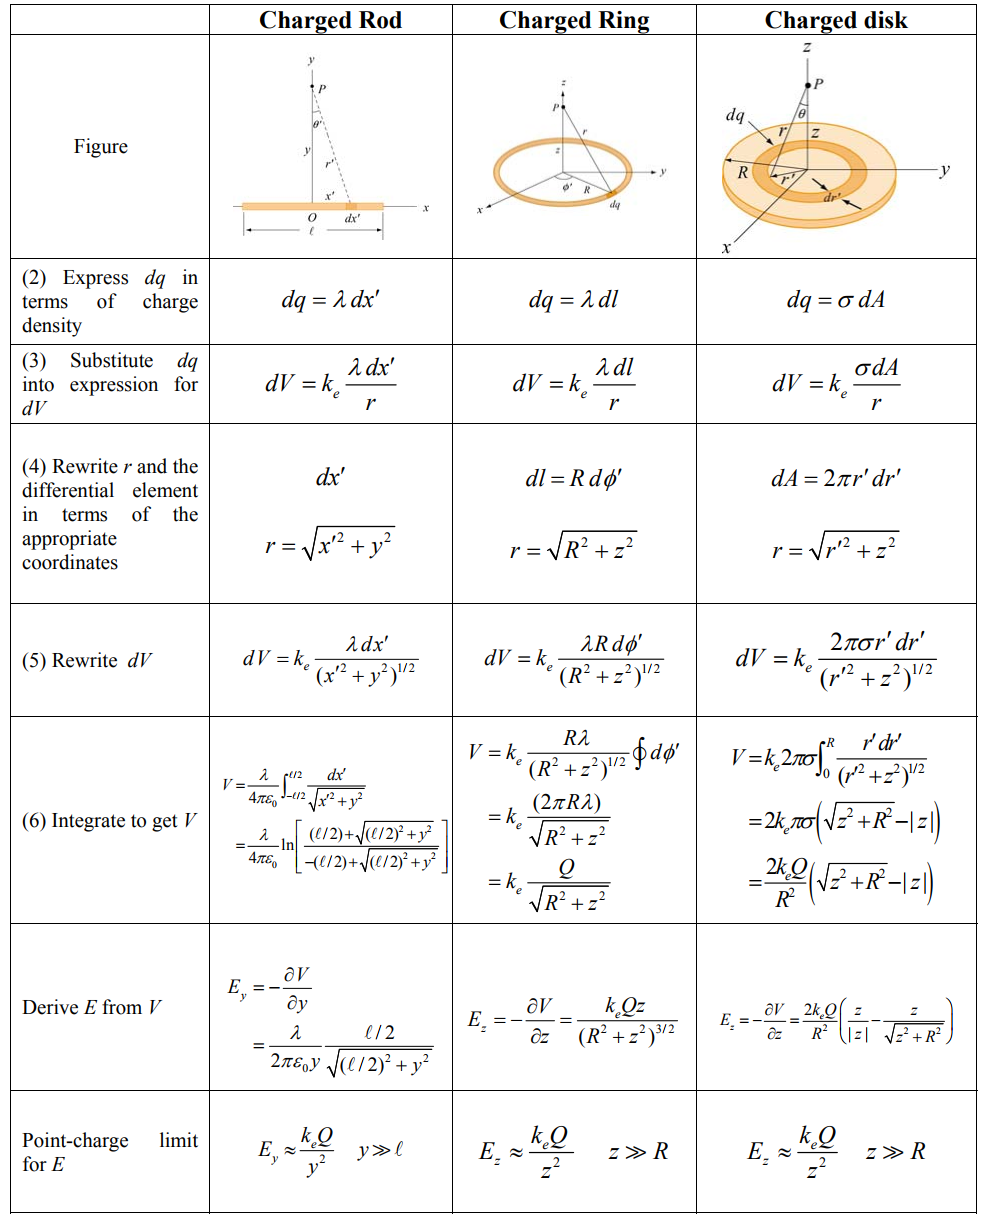
\includegraphics[width=\textwidth]{ExemplesPotElec.PNG}
\end{center}
















\section{Loi de Gauss}








\subsection{Théorie}







\begin{itemize}
    \item Le \textbf{flux électrique} qui passe au travers d'une surface caractérisée par le vecteur "zone" $ \vec{\textbf{A}} = A 
\hat{\textbf{n}} $ est: \[ \Phi_E = \vec{\textbf{E}} \cdot \vec{\textbf{A}} = E A \cos \theta \]
où $ \theta $ est l'angle entre le champ électrique $ \vec{\textbf{E}} $ et le vecteur unitaire $ \hat{\textbf{n}} $.
    \item En général, le flux électrique passant au travers d'une surface est: \[ \Phi_E = \iint_S \vec{\textbf{E}} \cdot d \vec{\textbf{A}} \]
    \item La \textbf{Loi de Gauss} affirme que le flux électrique passant au travers de n'importe quelle surface de Gauss est 
proportionnel à la charge totale enfermée par cette surface: \[ \Phi_E = \oiint_S \vec{\textbf{E}} \cdot d \vec{\textbf{A}} = \frac{q}{\epsilon_0} \]
La loi de Gauss peut être utilisée pour calculer le champ électrique d'un système qui possède une symétrie planaire, cylindrique ou sphérique.
    \item Les propriétés de base d'un \textbf{conducteur} sont: 
    \begin{enumerate}
        \item Le champ électrique au sein d'un conducteur est nul.
        \item Toute charge nette doit se trouver à la surface du conducteur.
        \item La surface d'un conducteur est une surface équipotentielle, et la composante tangentielle du champ électrique est nul à la surface.
        \item Juste à l'extérieur du conducteur, le champ électrique est normal à la surface.
    \end{enumerate}
    \item La \textbf{pression électrostatique} sur une surface conductrice est: \[ P = \frac{F}{A} = \frac{\sigma^2}{2 \epsilon_0} = 
\frac{1}{2} \epsilon_0 \Big( \frac{\sigma}{\epsilon_0} \Big)^2 = \frac{1}{2} \epsilon_0 E^2 \]
\end{itemize}
















\subsection{Pratique}






Comme expliqué dans la sous-section "Théorie", on a montré que l'on peut calculer le champ électrique grâce à la loi de Gauss: 
\[ \Phi_E = \oiint \vec{\textbf{E}} \cdot d \vec{\textbf{A}} = \frac{q}{\epsilon_0} \]

\begin{center}
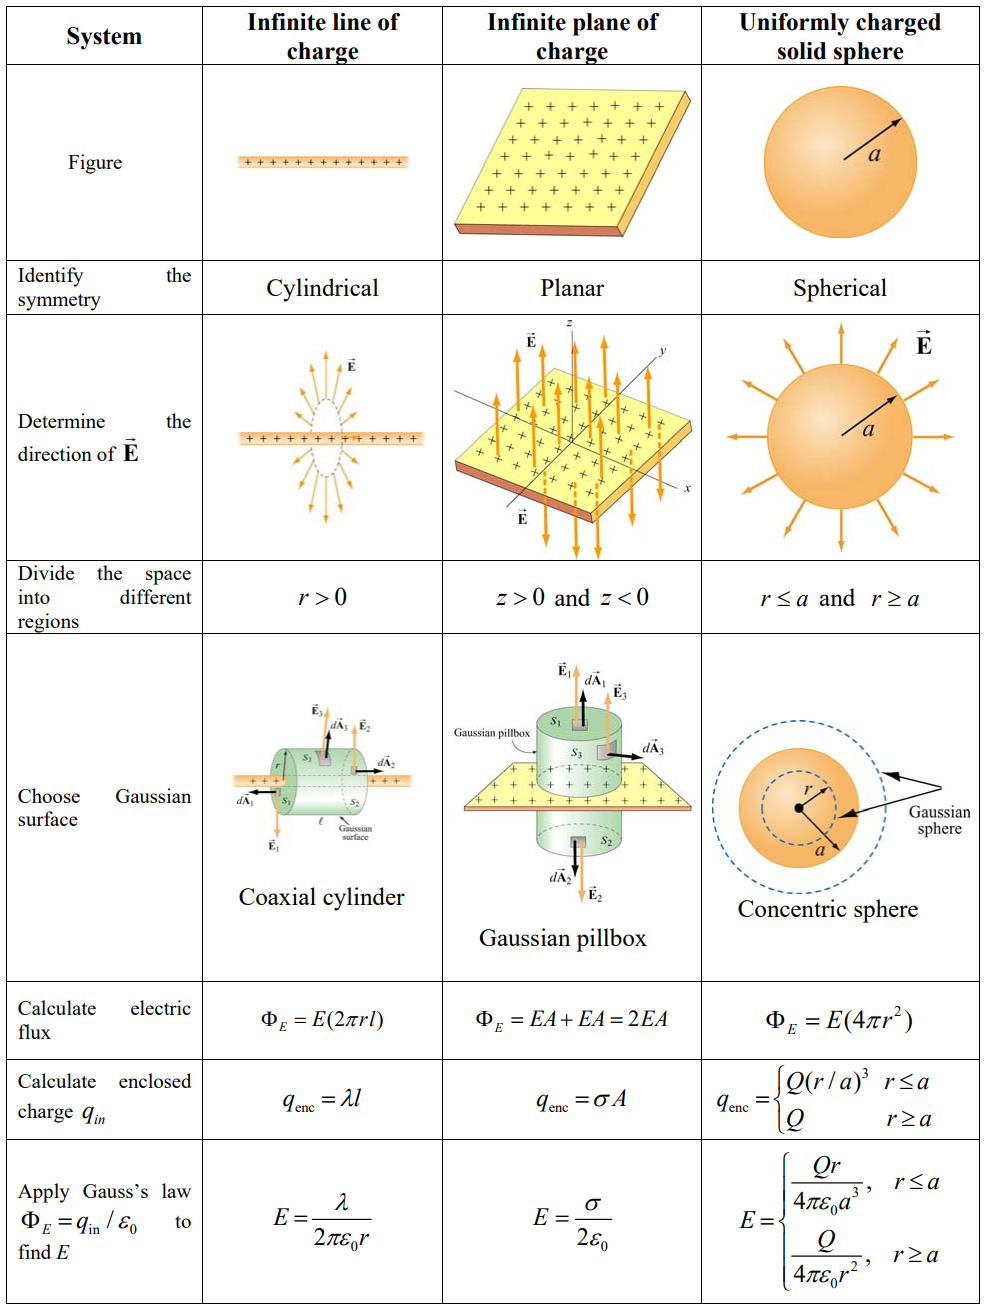
\includegraphics[width=\textwidth]{LoiGauss.PNG}
\end{center}























\section{Capacités et diélectriques}













\subsection{Théorie}







\begin{itemize}
    \item Un \textbf{condensateur} est un dispositif qui stocke des charges électriques et de l'énergie potentielle. La \textbf{capacité} $ C $ 
d'un condensateur est le ratio entre la charge stockée sur les plaques du condensateur et la différence de potentiel entre elles: 
\[ C = \frac{Q}{ | \Delta V | } \]
\begin{center}
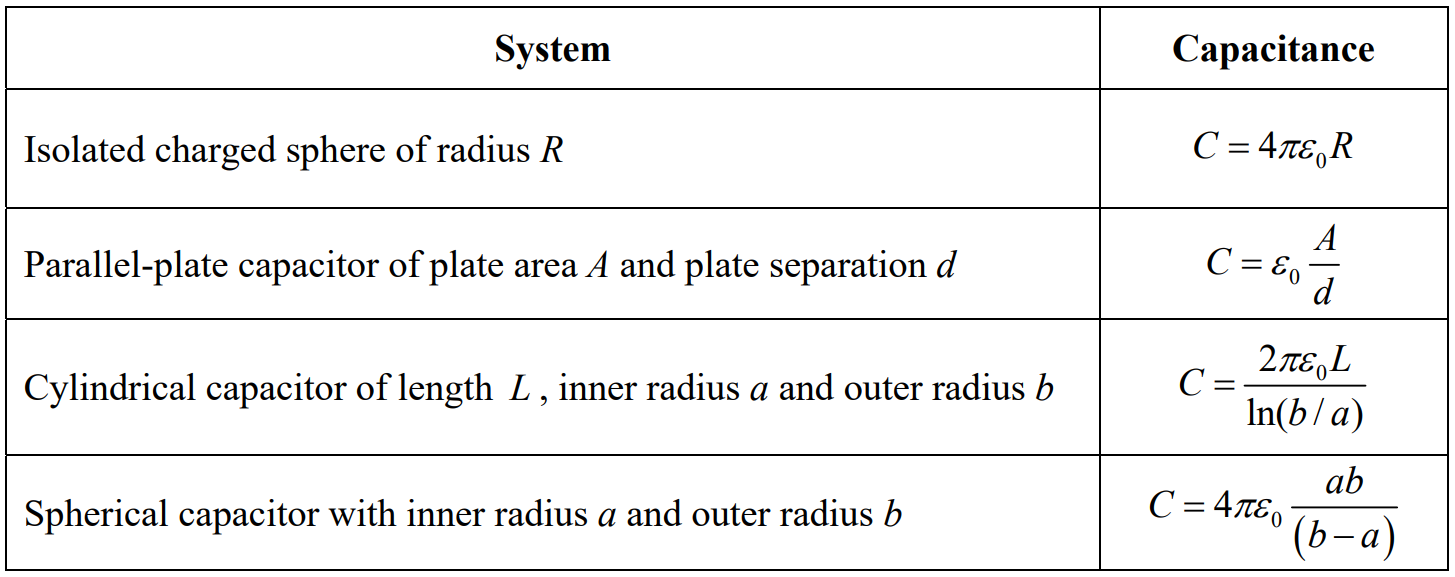
\includegraphics[width=0.8\textwidth]{capacite1.PNG}
\end{center}
    \item La capacité équivalente de condensateurs connectés en séries et en parallèles est: 
\[ C_T = C_1 + C_2 + C_3 + ... \qquad \text{ (parallèle) } \]
\[ \frac{1}{C_T} = \frac{1}{C_1} + \frac{1}{C_2} + \frac{1}{C_3} + ... \qquad \text{ (série) } \]
    \item Le travail réalisé pour charger un condensateur à une charge $ Q $ est: 
\[ U = \frac{Q^2}{2 C} = \frac{1}{2} Q | \Delta V | = \frac{1}{2} C | \Delta V |^2 \]
C'est égal à la quantité d'énergie stockée dans le condensateur.
    \item On peut aussi penser que l'énergie électrique est stockée dans le champ électrique $ \vec{\textbf{E}} $. La \textbf{densité 
énergétique} (énergie par unité de volume) est: \[ u_E = \frac{1}{2} \epsilon_0 E^2 \]
La densité énergétique $ u_E $ est égale à la \textbf{pression électrostatique} sur une surface.
    \item Lorsqu'un matériau diélectrique avec une \textbf{constante diélectrique} $ K_E $ est inséré dans un condensateur, la capacité 
est augmentée d'un facteur $ K_E $: \[ C = K_E C_0 \]
    \item Le vecteur de \textbf{polarisation} $ \vec{\textbf{P}} $ est le moment dipolaire par unité de volume (\danger \; moment 
dipolaire $ \neq $ moment de force): \[ \vec{\textbf{P}} = \frac{1}{V} \sum_{i=1}^{N} \vec{\textbf{p}}_i \]
Le champ électrique induit par la polarisation est: \[ \vec{\textbf{E}}_P = - \frac{\vec{\textbf{P}}}{\epsilon_0} \]
    \item En présence d'un diélectrique avec une constante diélectrique $ K_E $, le champ électrique devient: 
\[ \vec{\textbf{E}} = \vec{\textbf{E}}_0 + \vec{\textbf{E}}_p = \frac{\vec{\textbf{E}}_0}{K_E} \]
où  $ \vec{\textbf{E}}_0 $ est la valeur du champ électrique sans diélectrique.
\end{itemize}








\subsection{Pratique}






Voici la procédure pour calculer la capacité $ C $ de plusieurs systèmes: 
\begin{enumerate}
    \item Identifier la direction du champ électrique en utilisant la symétrie du système.
    \item Calculer le champ électrique partout.
    \item Calculer la différence de potentiel électrique $ | \Delta V | $.
    \item Calculer la capacité $ C $ en utilisant $\displaystyle C = \frac{Q}{| \Delta V |} $
\end{enumerate}

\begin{center}
    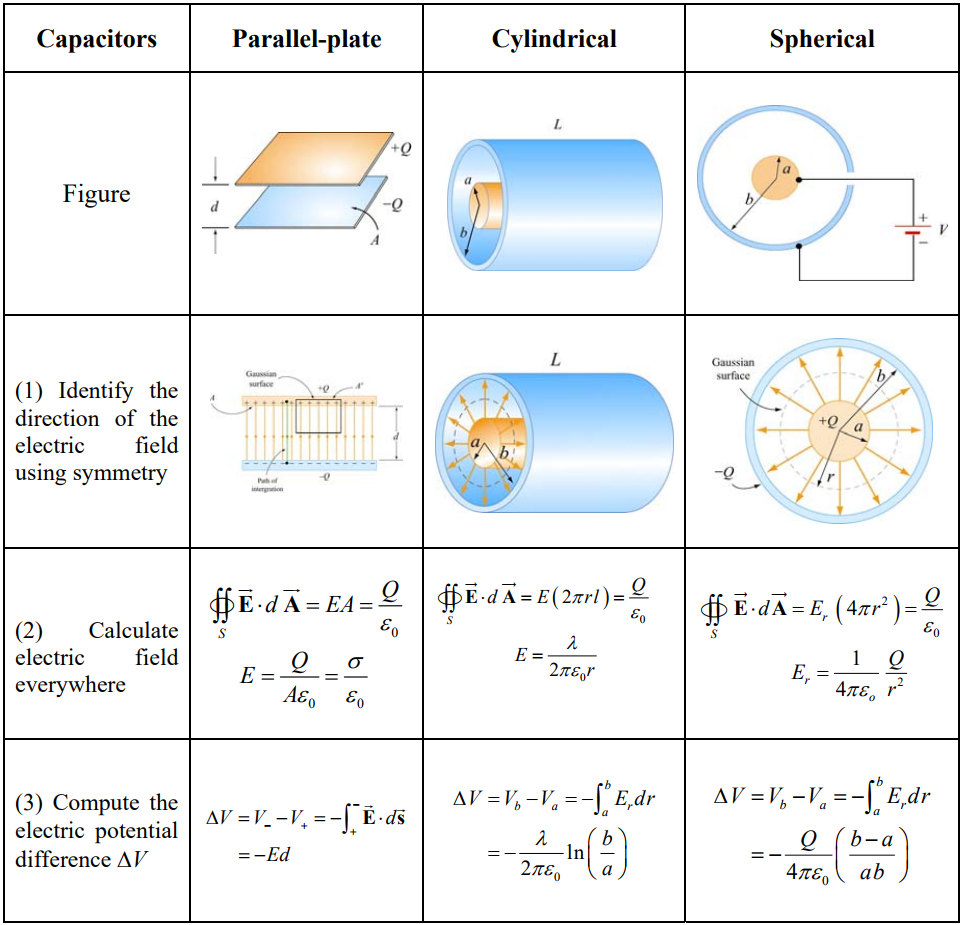
\includegraphics[width=\textwidth]{capacite2.PNG}
    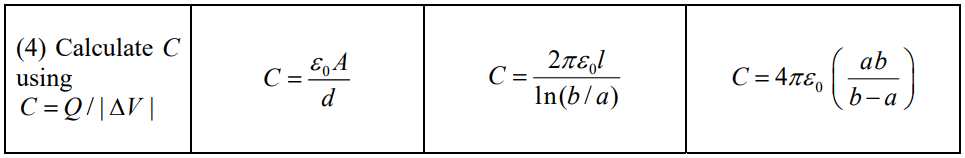
\includegraphics[width=\textwidth]{capacite3.PNG}
\end{center}

















\section{Courant et résistance}









\subsection{Théorie}






\renewcommand{\thefootnote}{\arabic{footnote}}
\begin{itemize}
    \item Le \textbf{courant électrique} est défini par: \[ I = \frac{d Q}{d t} \]
    \item Le courant moyen dans un conducteur est: \[ I_{moy} = n q v_d A \]
où $ n $ est la densité de porteurs de charge, $ q $ est la charge que chaque porteur possède, $ v_d $ est la vitesse de dérive (aussi appelée "vitesse de drift" est la vitesse moyenne d'un porteur de charge, ici un électron, atteinte sous l'effet d'un champ électrique $ \vec{\textbf{E}} $) et $ A $ est la surface en coupe transversale. \footnote{La charge totale d'une section vaut: $\displaystyle \Delta Q = q (n A \Delta x) $. Sur un intervalle de temps $ \Delta t $, on a: $ \Delta x = v_d \Delta t $. Ce qui implique que $\displaystyle I_{moy} = \frac{\Delta Q}{\Delta t} = n q v_d A $.}
\begin{center} 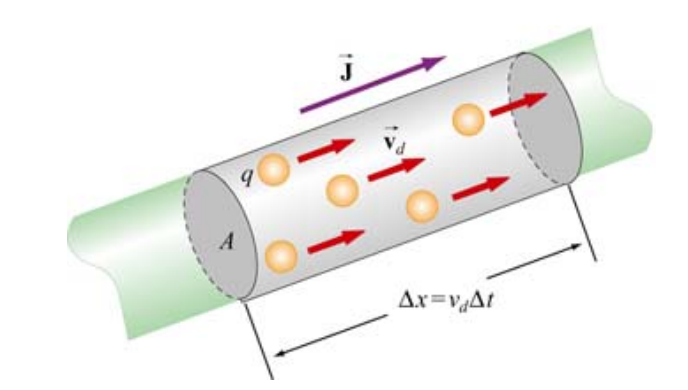
\includegraphics[width = 0.45\textwidth]{CourantNote.PNG} \end{center}
    \item La \textbf{loi d'Ohm} pour le microscopique: la densité de courant est proportionnelle au champ électrique, et la constante de 
proportionnalité $ \sigma $ est appelée conductivité: \[ \vec{\textbf{J}} = \sigma \vec{\textbf{E}} \]
    \item La réciproque de la conductivité $ \sigma $ est appelée \textbf{résistivité} $ \rho $: \[ \rho = \frac{1}{\sigma} \]
    \item La \textbf{loi d'Ohm} pour le macroscopique: La \textbf{résistance} $ R $ d'un conducteur est le ratio entre la différence de 
potentiel $ \Delta V $ (différence de potentiel entre les deux bouts du conducteur) et le courant $ I $: \[ R = \frac{\Delta V}{I} \]
    \item La résistance est reliée à la résistivité par: \[ R = \frac{\rho l}{A} \]
où $ l $ est la longueur et $ A $ est la surface en coupe transversale du conducteur.
    \item La \textbf{vitesse de dérive} d'un électron dans un conducteur est: \[ v_d = - \frac{e \vec{\textbf{E}}}{m_e} \tau \]
où $ e $ est la charge de l'électron, $ m_e $ sa masse et $ \tau $ est le temps moyen entre deux collisions successives.
    \item La résistivité d'un métal est reliée à $ \tau $ par: \[ \rho = \frac{1}{\sigma} = \frac{m_e}{n e^2 \tau} \]
    \item La variation de température de la résistance d'un conducteur est: 
\[ \rho = \rho_0 \Big[ 1 + \alpha (T - T_0) \Big] \]
où $ \alpha $ est le \textbf{coefficient de température de la résistance}.
    \item La \textbf{puissance} ou le débit auquel l'énergie est délivrée à la résistance est: 
\[ P = I \Delta V = I^2 R = \frac{( \Delta V )^2}{R} \]
\end{itemize}

















\section{Courant continu}











\subsection{Théorie}








\begin{itemize}
    \item La résistance équivalente à plusieurs résistances placées en série est: 
\[ R_T = R_1 + R_2 + R_3 + ... = \sum_{i=1}^{N} R_i \]
    \item La résistance équivalente à plusieurs résistances placées en parallèle est: 
\[ \frac{1}{R_T} = \frac{1}{R_1} + \frac{1}{R_2} + \frac{1}{R_3} + ... = \sum_{i=1}^{N} \frac{1}{R_i} \]
    \item \textbf{Lois de Kirchhoff}: 
    \begin{enumerate}
        \item La somme des courants entrants une jonction est égale à la somme des courants sortants de la jonction: 
        \[ \sum I_{in} = \sum I_{out} \]
        \item La somme algébrique des changements de potentiel électrique dans une boucle en circuit fermé est zéro. 
        \[ \sum_{\text{boucle fermée}} \Delta V = 0 \]
    \end{enumerate}
    \item Dans un condensateur en chargement, la charge et le courant en fonction du temps sont: 
\[ q(t) = Q \Big( 1 - e^{\frac{-t}{RC}} \Big), \qquad I(t) = \Big( \frac{\epsilon}{R} \Big) e^{\frac{-t}{RC}} \]
    \item  Dans un condensateur en déchargement, la charge et le courant en fonction du temps sont: 
\[ q(t) = Q e^{\frac{-t}{RC}}, \qquad I(t) = \Big( \frac{Q}{RC} \Big) e^{\frac{-t}{RC}} \]
\end{itemize}








\subsection{Pratique}






\textbf{Appliquer les lois de Kirchhoff}

La procédure pour analyser (résoudre) des circuits possédants plusieurs boucles est la suivante: 
\begin{enumerate}
    \item Tracer le diagramme du circuit, attribuer un symbole à toute les variables connues et inconnues. Le nombre d'inconnues 
correspond au nombre d'équations linéairement indépendantes que l'on doit trouver.
    \item Donner une direction au courant dans chaque branche du circuit (Si la vraie direction est opposée à celle que vous avez choisie,
la valeur du courant sera négative).
    \item Appliquer la loi des noeuds à toutes les jonctions sauf une (appliquer cette loi au dernier noeud ne donnera pas de relation
supplémentaire indépendante entre les courants).
    \item Appliquer la loi des boucles jusqu'à ce que le nombre d'équations indépendantes obtenues soit le même que le nombre d'inconnues.
\newline Par \emph{exemple}, si on a trois inconnues, il faut avoir trois équations linéairement indépendantes pour avoir une solution unique.
\begin{center} 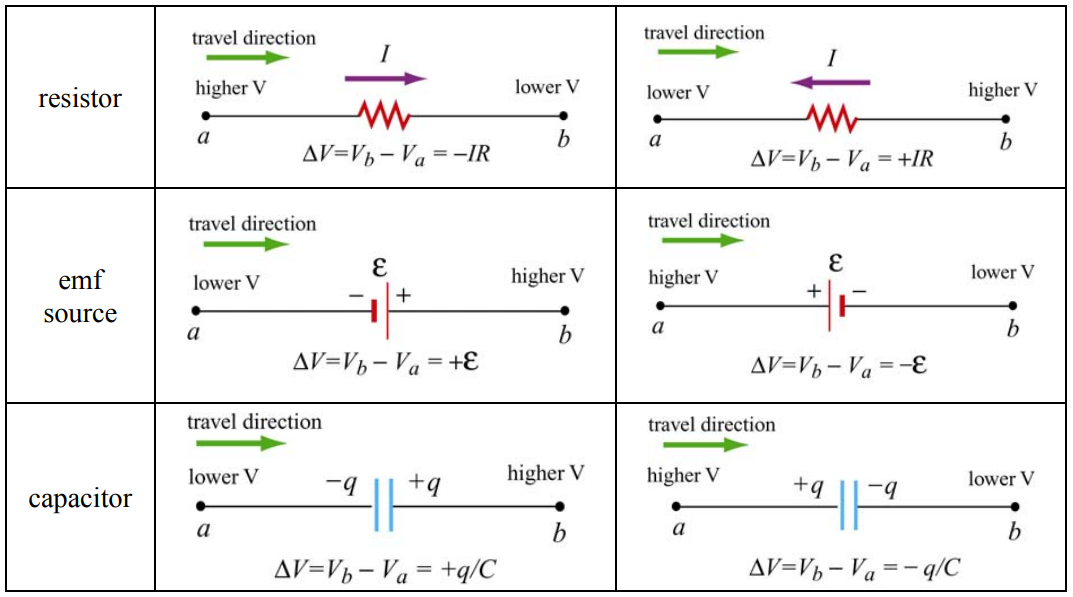
\includegraphics[width=0.8\textwidth]{Kirchhoff.PNG} \end{center}
Notez que la même équation est obtenue que vous parcouriez la boucle dans le sens horloger ou anti-horloger.
    \item Résoudre simultanément toutes les équations pour obtenir les solutions de toutes les inconnues.
\end{enumerate}



















\section{Introduction aux champs magnétiques}










\subsection{Théorie}









\begin{itemize}
    \item La \textbf{force magnétique} agissant sur une charge $ q $ se déplaçant à une vitesse $ \vec{\textbf{v}} $ dans un champ 
magnétique $ \vec{\textbf{B}} $ est donnée par: \[ \vec{\textbf{F}}_B = q \vec{\textbf{v}} \wedge \vec{\textbf{B}} \]
    \item La force magnétique agissant sur un conducteur de longueur $ \vec{\textbf{l}} $ traversé par un courant $ I $ dans un champ 
magnétique $ \vec{\textbf{B}} $ est: \[ \vec{\textbf{F}}_B = I \; \vec{\textbf{l}} \wedge \vec{\textbf{B}} \]
    \item La force magnétique $ d \vec{\textbf{F}}_B $ générée par une petite portion du courant $ I $ de longueur $ d \vec{\textbf{s}} $ 
dans un champ magnétique $ \vec{\textbf{B}} $ est: 
\[ d \vec{\textbf{F}}_B = I \; d \vec{\textbf{s}} \wedge \vec{\textbf{B}} \]
    \item Le \textbf{moment de force} $ \vec{\boldsymbol{\tau}} $ agissant sur une boucle fermée conductrice d'aire $ A $ et traversée par
un courant $ I $ dans un champ magnétique uniforme $ \vec{\textbf{B}} $ est: 
\[ \vec{\boldsymbol{\tau}} = I \vec{\textbf{A}} \wedge \vec{\textbf{B}} \]
où $ \vec{\textbf{A}} $ est un vecteur de grandeur $ A $ et une direction perpendiculaire à la boucle.
    \item Le \textbf{moment magnétique dipolaire} (encore une fois, moment magnétique dipolaire $ \neq $ moment de force) d'une boucle 
fermée conductrice d'aire $ A $ traversée par un courant $ I $ est donnée par: 
\[ \vec{\boldsymbol{\mu}} = I \vec{\textbf{A}} \]
    \item Le moment de force exercée sur un dipôle magnétique $ \vec{\boldsymbol{\tau}} $ placé dans un champ magnétique extérieur $ 
\vec{\textbf{B}} $ est: \[ \vec{\boldsymbol{\tau}} = \vec{\boldsymbol{\mu}} \wedge \vec{\textbf{B}} \]
    \item L'énergie potentielle d'un dipôle magnétique placé dans un champ magnétique est: 
\[ U = - \vec{\boldsymbol{\mu}} \cdot \vec{\textbf{B}} \]
    \item Si une particule de charge $ q $ et de masse $ m $ entre dans un champ magnétique de magnitude $ B $ avec une vitesse $ 
\vec{\textbf{v}} $ perpendiculaire aux lignes de champ magnétique, le rayon du chemin circulaire suivit par la particule est: 
\[ r = \frac{m v}{|q| B} \]
et la vitesse angulaire de la particule est: $\displaystyle \omega = \frac{|q| B}{m} $.
\end{itemize}










\subsection{Aide pour la pratique}







Dans la sous-section "Théorie", il est expliqué que en présence du champ magnétique $ \vec{\textbf{B}} $ et du champ électrique $ \vec{\textbf{E}} $, la force totale agissant sur une particule en mouvement de charge $ q $ est: $\displaystyle \vec{\textbf{F}} = \vec{\textbf{F}}_e + \vec{\textbf{F}}_B = q (\vec{\textbf{E}} + \vec{\textbf{v}} \wedge \vec{\textbf{B}}) $, où $ \vec{\textbf{v}} $ est la vitesse de la particule. La direction de $ \vec{\textbf{F}}_B $ implique le produit vectoriel de $ \vec{\textbf{v}} $ et de $ \vec{\textbf{B}} $, qui se base sur la règle de la main droite. En coordonnées cartésiennes, les vecteurs unitaires sont $ \hat{\textbf{i}} $, $ \hat{\textbf{j}} $ et $ \hat{\textbf{k}} $ qui satisfont les propriétés suivantes: 
\[ \hat{\textbf{i}} \wedge \hat{\textbf{j}} = \hat{\textbf{k}}, \qquad \hat{\textbf{j}} \wedge \hat{\textbf{k}} = \hat{\textbf{i}}, \qquad \hat{\textbf{k}} \wedge \hat{\textbf{i}} = \hat{\textbf{j}} \]
\[ \hat{\textbf{j}} \wedge \hat{\textbf{i}} = - \hat{\textbf{k}}, \qquad \hat{\textbf{k}} \wedge \hat{\textbf{j}} = - \hat{\textbf{i}}, \qquad \hat{\textbf{i}} \wedge \hat{\textbf{k}} = - \hat{\textbf{j}} \]
\[ \hat{\textbf{i}} \wedge \hat{\textbf{i}} = \hat{\textbf{j}} \wedge \hat{\textbf{j}} = \hat{\textbf{k}} \wedge \hat{\textbf{k}} = \vec{\textbf{0}} \]
Pour $ \vec{\textbf{v}} = v_x \hat{\textbf{i}} + v_y \hat{\textbf{j}} + v_z \hat{\textbf{k}} $ et $ \vec{\textbf{B}} = B_x \hat{\textbf{i}} + B_y \hat{\textbf{j}} + B_z \hat{\textbf{k}} $ le produit vectoriel peut être obtenu ainsi: 
\[ \vec{\textbf{v}} \wedge \vec{\textbf{B}} = 
\begin{vmatrix}
\hat{\textbf{i}} & \hat{\textbf{j}} & \hat{\textbf{k}} \\
v_x & v_y & v_z \\
B_x & B_y & B_z
\end{vmatrix}
= (v_y B_z - v_z B_y) \hat{\textbf{i}} + (v_z B_x - v_x B_z) \hat{\textbf{j}} + (v_x B_y - v_y B_x) \hat{\textbf{k}} \]
Si seulement le champ magnétique est présent, et si $ \vec{\textbf{v}} $ est perpendiculaire à $ \vec{\textbf{B}} $, alors la trajectoire est un cercle de rayon $\displaystyle r = \frac{m v}{|q| B} $ et la vitesse angulaire est $\displaystyle \omega = \frac{|q| B}{m} $.

Lorsque l'on a affaire à un cas plus compliqué, il est utile de travailler avec les composantes de la force. Par exemple: 
$\displaystyle F_x = m a_x = q E_x + q (v_y B_z - v_z B_y) $.






















\section{Sources de champ magnétique}











\subsection{Théorie}







\begin{itemize}
    \item La \textbf{loi de Biot-Savart} déclare que le champ magnétique $ d \vec{\textbf{B}} $ en un point et dû à un élément de longueur
$ d \vec{\textbf{s}} $ traversé par un courant continu $ I $ et localisé à la distance donnée par $ \vec{\textbf{r}} $ est donné par: 
\[ d \vec{\textbf{B}} = \frac{\mu_0}{4 \pi} \frac{I d \vec{\textbf{s}} \wedge \vec{\textbf{r}}}{r^2} \]
où $ r = \| \vec{\textbf{r}} \| $ et $ \mu_0 = 4 \pi \times 10^{-7} T m / A $ est la permittivité du vide.
    \item La magnitude du champ magnétique à une distance $ r $ d'un fil conducteur rectiligne infiniment long traversé par un courant $ I
$ est: \[ B = \frac{\mu_0 I}{2 \pi R} \]
    \item La magnitude de la force magnétique $ F_B $ entre deux fils rectilignes de longueur $ l $ traversés par des courants continus 
$ I_1 $ et $ I_2 $ et séparés par une distance $ r $ est: 
\[ F_B = \frac{\mu_0 I_1 I_2 l}{2 \pi r} \]
    \item La \textbf{loi d'Ampère} déclare que l'intégrale curviligne de $ \vec{\textbf{B}} \cdot d \vec{\textbf{s}} $ autour de n'importe
quelle boucle est proportionnel au courant continu total traversant n'importe quelle surface délimitée par cette boucle: 
\[ \oint \vec{\textbf{B}} \cdot d \vec{\textbf{s}} = \mu_0 I \]
     \item Le champ magnétique au sein d'un \textbf{toroïde} qui possède $ N $ boucles étroitement espacées traversées par un courant 
$ I $ est donné par \[ B = \frac{\mu_0 N I}{2 \pi R} \]
où $ r $ est la distance jusqu'au centre du \textbf{toroïde}.
    \item Le champ magnétique au centre d'un \textbf{solénoïde} possédant $ N $ boucles étroitement espacées traversées par un courant 
$ I $ sur une longueur $ l $ est donné par: 
\[ B = \mu_0 \frac{N}{l} I = \mu_0 n I \]
où $ n $ est le nombre de boucles par unité de longueur.
    \item Les propriétés des matériaux magnétiques sont les suivantes: 
\begin{center} 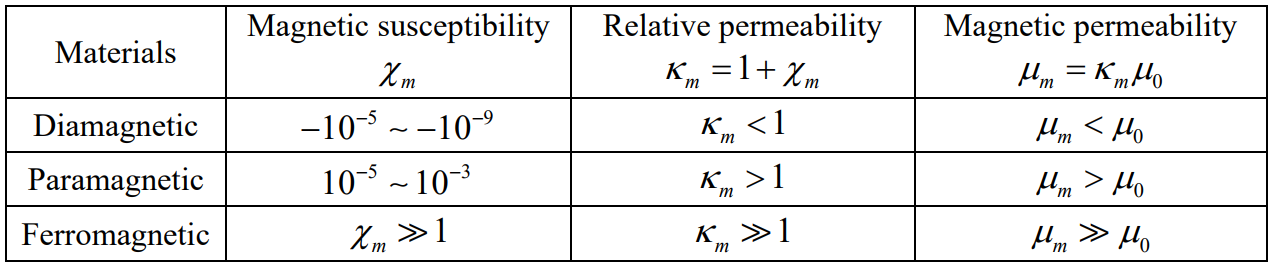
\includegraphics[width=0.8\textwidth]{PropMateriaux.PNG} \end{center}
\end{itemize}















\subsection{Pratique}







Dans la partie "Théorie", il est dit que l'on peut utiliser les lois de Biot-Savart et d'Ampère pour calculer le champ magnétique dû à une source électrique.





\subsubsection{Loi de Biot-Savart}




La loi déclare que le champ magnétique en un point $ P $ dû à un élément de longueur $ d \vec{\textbf{s}} $ traversé par un courant continu $ I $ est donné par: 
\[ d \vec{\textbf{B}} = \frac{\mu_0 I}{4 \pi} \frac{d \vec{\textbf{s}} \wedge \hat{\textbf{r}}}{r^2} = \frac{\mu_0 I}{4 \pi} \frac{d \vec{\textbf{s}} \wedge \vec{\textbf{r}}}{r^3} \]
Le calcul du champ magnétique peut se faire de la manière suivante: 
\begin{enumerate}
    \item \emph{\underline{Source}}: Choisir un système de coordonnées approprié et écrire une expression pour l'élément de courant 
différentiel $ I \; d \vec{\textbf{s}} $, et pour le vecteur $ \overrightarrow{\textbf{r'}} $ décrivant la position de $ I \; d \vec{\textbf{s}} $. La magnitude $ r' = \| \overrightarrow{\textbf{r'}} \| $ est la distance entre $ I \; d \vec{\textbf{s}} $ et l'origine. Les variables avec un "prime" sont utilisées pour la source.
    \item \emph{\underline{Point du champ}}: Le point $ P $ est un point de l'espace où le champ magnétique dû au courant doit être 
calculé. En utilisant le même système de coordonnées, écrire le vecteur position $ \vec{\textbf{r}}_p $ pour le point $ P $. La quantité $ r_p = \| \vec{\textbf{r}}_p \| $ est la distance entre l'origine et $ P $.
    \item \emph{\underline{Vecteur de position relative}}: La position relative entre la source et le point est caractérisée par le 
vecteur de position relative $ \vec{\textbf{r}} = \vec{\textbf{r}}_p - \overrightarrow{\textbf{r'}} $. Le vecteur unitaire correspondant est: 
\[ \hat{\textbf{r}} = \frac{\vec{\textbf{r}}}{r} = \frac{\vec{\textbf{r}}_p - \overrightarrow{\textbf{r'}}}{\| \vec{\textbf{r}}_p - \overrightarrow{\textbf{r'}} \|} \]
où $ r = \| \vec{\textbf{r}} \| = \| \vec{\textbf{r}}_p - \overrightarrow{\textbf{r'}} \| $ est la distance entre la source et le point $ P $.
    \item Calculer le produit vectoriel $ d \vec{\textbf{s}} \wedge \overrightarrow{\textbf{r}} $ ou $ d \vec{\textbf{s}} \wedge 
\vec{\textbf{r}} $. Le vecteur résultant donne la direction du champ magnétique $ \vec{\textbf{B}} $, selon la loi de Biot-Savart.
    \item Substituer les expressions obtenues dans $ d \vec{\textbf{B}} $ et simplifier autant que possible.
    \item Compléter l'intégration pour obtenir $ \vec{\textbf{B}} $ si possible. La taille et la géométrie du système se reflètent dans 
les limites d'intégration. Changer les variables d'intégration peut parfois aider à compléter l'intégration.
\end{enumerate}

\begin{center}
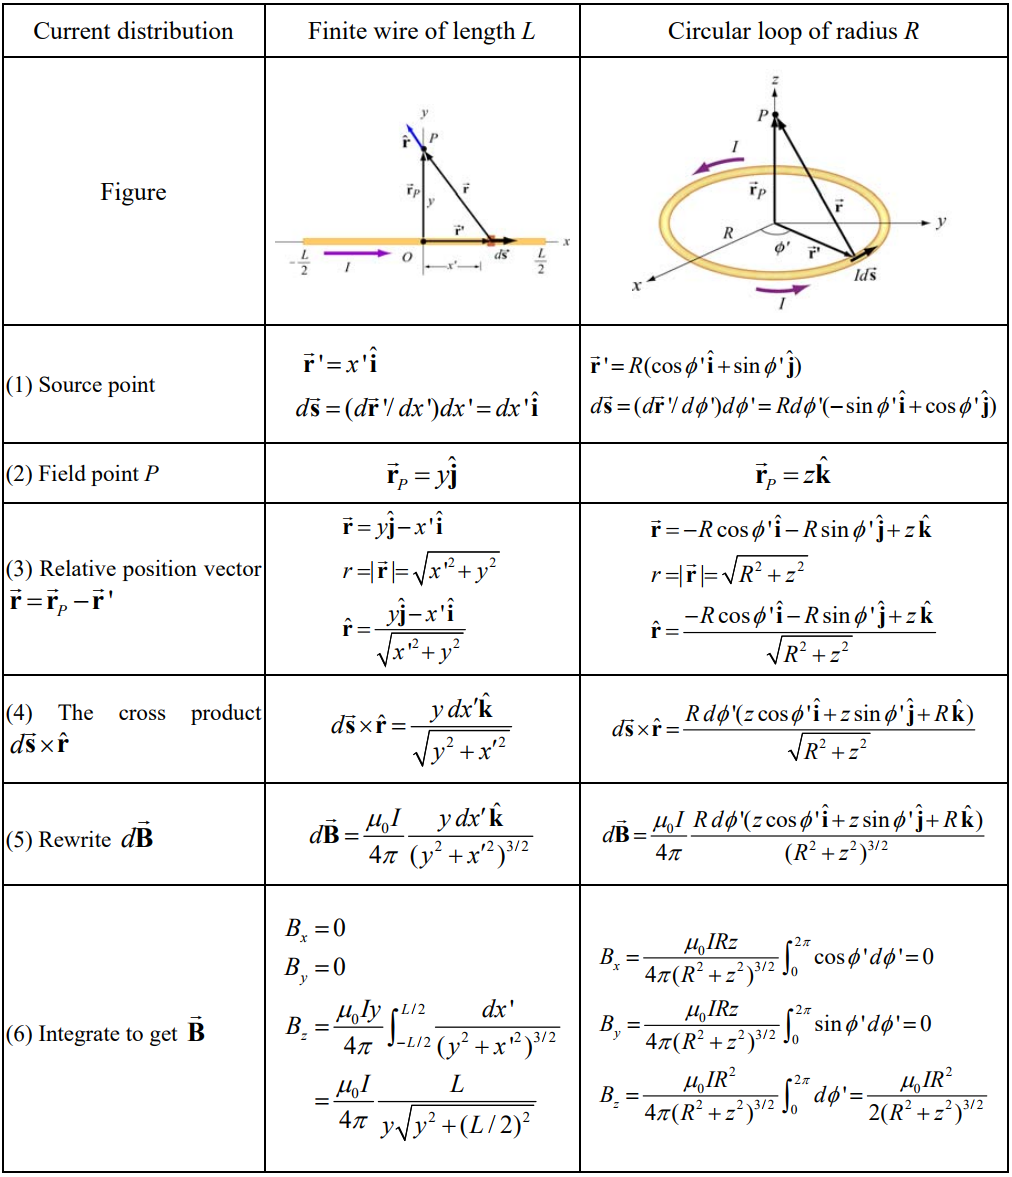
\includegraphics[width=\textwidth]{MagneticField.PNG}
\end{center}







\newpage







\subsubsection{Loi d'Ampère}






La loi d'Ampère déclare que l'intégrale curviligne de $ \vec{\textbf{B}} \cdot d \vec{\textbf{s}} $ autour d'une boucle fermée est proportionnel au courant total passant au travers de n'importe quelle surface délimitée par cette boucle fermée: 
\[ \oint \vec{\textbf{B}} \cdot d \vec{\textbf{s}} = \mu_0 I \]
On applique la loi d'Ampère pour calculer le champ magnétique selon la procédure suivante: 
\begin{enumerate}
    \item Dessiner une boucle "ampèrienne" en utilisant des arguments de symétrie (le courant doit passer au travers de la boucle).
    \item Trouver le courant passant au travers de la boucle.
    \item Calculer l'intégrale curviligne $ \oint \vec{\textbf{B}} \cdot d \vec{\textbf{s}} $ autour de la boucle fermée.
    \item Égaliser $ \oint \vec{\textbf{B}} \cdot d \vec{\textbf{s}} $ avec $ \mu_0 I $ et résoudre pour $ \vec{\textbf{B}} $.
\end{enumerate}
\begin{center}
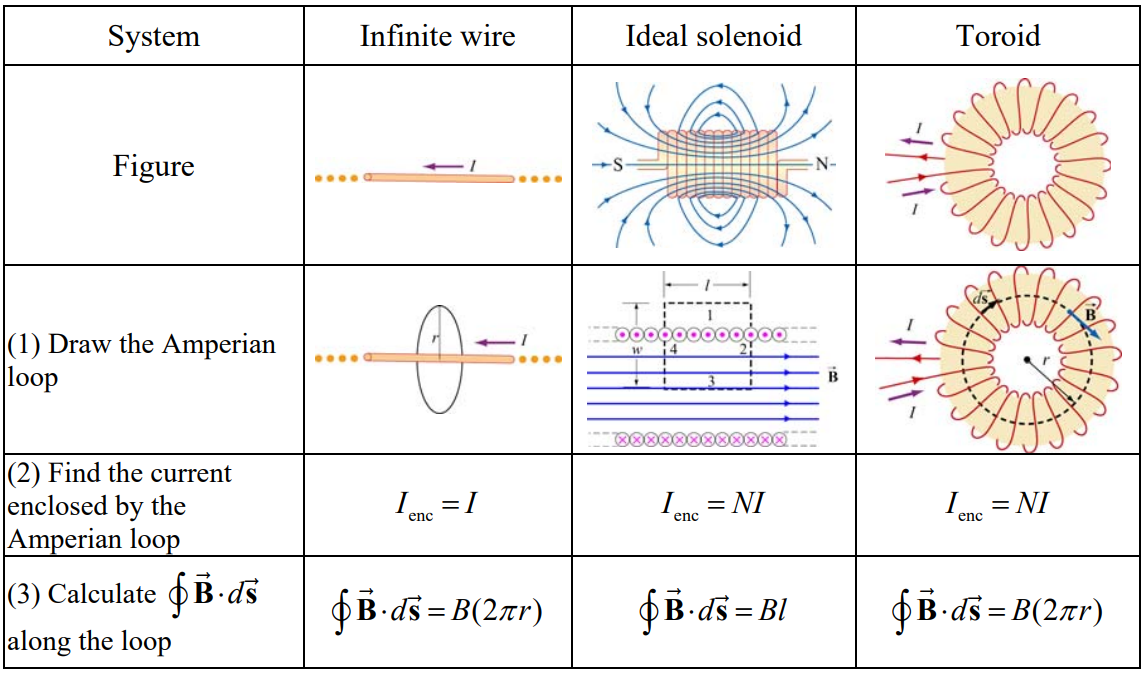
\includegraphics[width=\textwidth]{Ampere1}
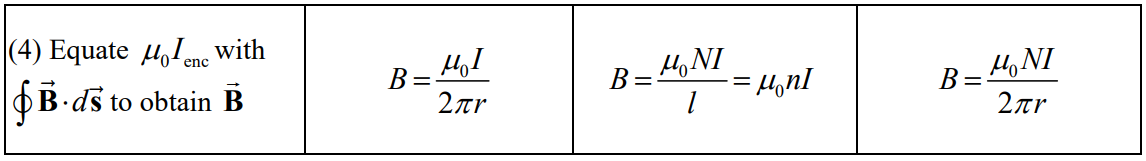
\includegraphics[width=\textwidth]{Ampere2}
\end{center}




















\section{Loi d'induction de Faraday}











\subsection{Théorie}







\begin{itemize}
    \item Le \textbf{flux magnétique} traversant une surface $ S $ est donné par: 
\[ \Phi_B = \iint_S \vec{\textbf{B}} \cdot d \vec{\textbf{A}} \]
    \item La \textbf{Loi de Faraday} (loi d'induction de Faraday) déclare que la fem $ \epsilon $ (fem = force électromotrice) induite 
dans une bobine est proportionnel à l'opposé de la vitesse du changement du flux magnétique: 
\[ \epsilon = - N \frac{d \Phi_B}{d t} \]
    \item La direction du courant induit est déterminé par la \textbf{loi de Lenz} qui déclare que le courant induit produit des champs 
magnétiques qui ont tendance à opposer le flux magnétique qui les a induits.
    \item Une \textbf{fem induite} est induite si un conducteur se déplace dans un champ magnétique. L'expression générale pour 
$ \epsilon $ est: 
\[ \epsilon = \oint \Big( \vec{\textbf{v}} \wedge \vec{\textbf{B}} \Big) \cdot d \vec{\textbf{s}} \]
Dans ce cas, une barre conductrice de longueur $ l $ se déplaçant à une vitesse constante $ \vec{\textbf{v}} $ dans un champ magnétique qui pointe dans la direction perpendiculaire à la barre et $ \vec{\textbf{v}} $, la fem induite est: $ \epsilon = - B v l $.
    \item Une fem induite dans un conducteur stationnaire est associée avec un champ électrique non-conservatif $ E_{nc} $: 
\[ \epsilon = \oint \vec{\textbf{E}}_{nc} \cdot d \vec{\textbf{s}} = - \frac{d \Phi_B}{d t} \]
\end{itemize}

















\subsection{Aide pour la pratique}







\emph{\textbf{Loi de Faraday et Loi de Lenz}}: 

Dans la partie "Théorie", nous avons vu que le changement de flux magnétique induit une fem: $\displaystyle \epsilon = - N \frac{d \Phi_B}{d t} $ d'après la loi d'induction de Faraday. Pour un conducteur qui forme une boucle fermée, la fem induit un courant $\displaystyle I = \frac{| \epsilon |}{R} $, où $ R $ est la résistance de la boucle. Pour calculer le courant induit et sa direction, on suit la procédure suivante: 
\begin{enumerate}
    \item Pour une boucle fermée d'aire $ A $ sur un plan, définir un vecteur surface $ \vec{\textbf{A}} $ qui pointe dans la direction
de votre pouce, pour pouvoir appliquer la règle de la main droite plus tard. Calculer le flux magnétique au travers de la boucle en utilisant: 
\[ \Phi_B = 
\begin{cases}
\vec{\textbf{B}} \cdot \vec{\textbf{A}}                 & \text{ ($ \vec{\textbf{B}} $ est uniforme) } \\ \displaystyle
\iint \vec{\textbf{B}} \cdot d \vec{\textbf{A}}         & \text{ ($ \vec{\textbf{B}} $ est non-uniforme) }
\end{cases}
\]
Déterminer le signe de $ \Phi_B $.
    \item Évaluer la vitesse de changement du flux magnétique $\displaystyle \frac{d \Phi_B}{d t} $. Il faut garder à l'esprit que le
changement peut être causé par 
\begin{enumerate}[i.]
    \item une variation du champ magnétique: $\displaystyle \frac{d B}{d t} \neq 0 $
    \item un changement de l'aire de la boucle si le conducteur est en mouvement $\displaystyle \Big( \frac{d A}{d t} \neq 0 \Big) $
    \item un changement d'orientation de la boucle par rapport au champ magnétique $\displaystyle \Big( \frac{d \theta}{d t} \neq 0 \Big) $
\end{enumerate}
Déterminer le signe de $\displaystyle \frac{d \Phi_B}{d t} $.
    \item Le signe de la fem induite est de signe opposé à $\displaystyle \frac{d \Phi_B}{d t} $. La direction du courant induit peut être trouvée en utilisant la loi de Lenz.
\end{enumerate}





















\section{Inductance et énergie magnétique}









\subsection{Théorie}







\begin{itemize}
    \item En utilisant la loi d'induction de Faraday, l'\textbf{inductance mutuelle} de deux bobines est donnée par: 
\[ M_{12} = \frac{N_1 \Phi_{12}}{I_2} = M_{21} = \frac{N_2 \Phi_{21}}{I_1} \]
où $ N_1 $ est le nombre de boucle de la bobine 1, $ I_1 $ est le courant qui la traverse, $ \Phi_{21} $ est le flux magnétique traversant UNE boucle de la bobine 2 et causé par $ I_1 $.
    \item La fem induite dans la bobine 2 par un changement de courant dans la bobine 1 est donnée par: 
\[ \epsilon_2 = - M \frac{d I_1}{d t} \]
    \item La \textbf{self-inductance} d'une bobine à $ N $ boucle est: 
\[ L = \frac{N \Phi_B}{I} \]
où $ \Phi_B $ est le flux magnétique traversant une boucle de la bobine.
    \item La fem auto-induite (self-induced) répondant à un changement de courant au sein de la bobine est: 
\[ \epsilon_L = - L \frac{d I}{d t} \]
    \item L'inductance d'un solénoïde à $ N $ boucles avec une aire de section transversale égale à $ A $ et de longueur $ l $ est: 
\[ L = \frac{\mu_0 N^2 A}{l} \]
    \item Si une batterie alimentant le circuit par une fem $ \epsilon $ est connecté à un solénoïde (solénoïde = bobine = 
auto-inductance = "self") et à une résistance en série à un temps $ t = 0 $, le courant dans ce \textbf{circuit RL} en fonction du temps est: \[ I(t) = \frac{\epsilon}{R} \Big( 1 - e^{\frac{-t}{\tau}} \Big) \]
où $ \tau = L / R $ est la constante de temps du circuit. Si la batterie est retirée du circuit RL, le courant va diminuer selon: 
\[ I(t) = \Big( \frac{\epsilon}{R} \Big) e^{\frac{-t}{\tau}} \]
    \item L'\textbf{énergie magnétique} stockée dans un solénoïde traversé par un courant $ I $ est: 
\[ U_B = \frac{1}{2} L I^2 \]
    \item La \textbf{densité d'énergie magnétique} en un point avec un champ magnétique $ B $ est: 
\[ u_B = \frac{B^2}{2 \mu_0} \]
    \item L'équation différentielle pour un \textbf{circuit LC} oscillant est: 
\[ \frac{d^2 Q}{d t^2} + \omega_0^2 Q = 0 \]
où $\displaystyle \omega_0 = \frac{1}{\sqrt{LC}} $ est la fréquence angulaire d'oscillation. La charge du condensateur en fonction du temps est donné par: 
\[ Q(t) = Q_0 \cos (\omega_0 t + \phi) \]
et le courant dans le circuit est: 
\[ I(t) = - \frac{d Q}{d t} = + \omega_0 Q_0 \sin (\omega_0 t + \phi) \]
    \item L'énergie totale dans un circuit LC est, en utilisant $\displaystyle I_0 = \omega_0 Q_0 $, 
\[ U = U_E + U_B = \frac{Q_0^2}{2 C} \cos^2 \omega_0 t + \frac{L I_0^2}{2} \sin^2 \omega_0 t = \frac{Q_0^2}{2 C} \]
    \item L'équation différentielle pour un \textbf{circuit RLC} est: 
\[ \frac{d^2 Q}{d t^2} + 2 \gamma \frac{d Q}{d t} + \omega_0^2 Q = 0 \]
où $\displaystyle \omega_0 = \frac{1}{\sqrt{LC}} $ et $\displaystyle \gamma = \frac{R}{2 L} $. Dans ce cas, la charge du condensateur en fonction du temps est: 
\[ Q(t) = Q_0 e^{- \gamma t} \cos (\omega ' t + \phi) \]
où $\displaystyle \omega ' = \sqrt{\omega_0^2 - \gamma^2} $.
\end{itemize}
















\subsection{Pratique}









\subsubsection{Calculer la self-inductance}







La self-inductance $ L $ d'une bobine peut être calculée en suivant la procédure suivante: 
\begin{enumerate}
    \item Supposer un courant constant $ I $ pour l'inducteur, l'inducteur pouvant être une boucle conductrice, un solénoïde, un toroïde 
ou des câbles coaxiaux.
    \item Choisir une section transversale appropriée $ S $ et calcule le flux magnétique traversant $ S $ en utilisant: 
\[ \Phi_B = \iint_S \vec{\textbf{B}} \cdot d \vec{\textbf{A}} \]
Si la surface est délimitée par $ N $ tours de fils (il y a $ N $ boucles), alors le flux magnétique total à travers la surface est: $\displaystyle N \Phi_B $.
    \item L'inductance peut être obtenue avec: 
\[ L = \frac{N \Phi_B}{I} \]
\end{enumerate}








\subsubsection{Circuits contenant des inducteurs}







Trois types de circuits à boucle unique ont été examinés dans cette section: RL, LC et RLC. Pour mettre en place l'équation différentielle du circuit, on applique la loi des boucles et des noeuds de Kirchhoff, comme pour les circuits RC. Pour les circuits contenant des inducteurs, la règle de Kirchhoff modifiée correspondante est schématisée ci-dessous.
\begin{center}
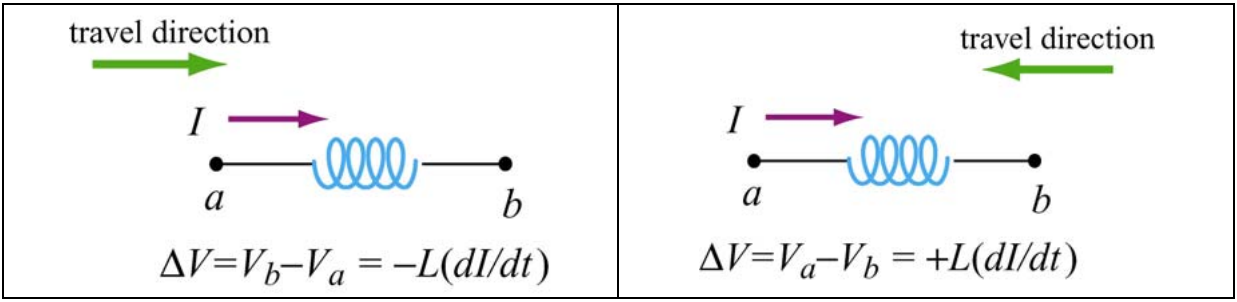
\includegraphics[width=0.8\textwidth]{inductance.PNG}
\end{center}
Remarque: la "différence de potentiel" entre les deux bouts de l'inducteur est proportionnelle au taux de variation du courant $\displaystyle \frac{d I}{d t} $. La situation se simplifie si on est seulement intéressé dans le comportement à long terme du circuit, lorsque le courant sera stable $\displaystyle \frac{d I}{d t} = 0 $. Dans cette limite, l'inducteur peut être remplacé par un fil conducteur normal.

























\section{Courant alternatif}









\subsection{Théorie}








\begin{itemize}
    \item Dans un circuit AC avec une source de tension sinusoïdale $ V(t) = V(0) \sin \omega t $, le courant est donné par 
$ I(t) = I_0 \sin (\omega t - \phi) $, où $ I_0 $ est l'amplitude et $ \phi $ est le déphasage (aussi appelé phase à l'origine). Pour un circuit simple avec seulement un composant (une résistance, un condensateur ou un inducteur), connecté à la source de tension, les résultats sont les suivants: 
\begin{center}
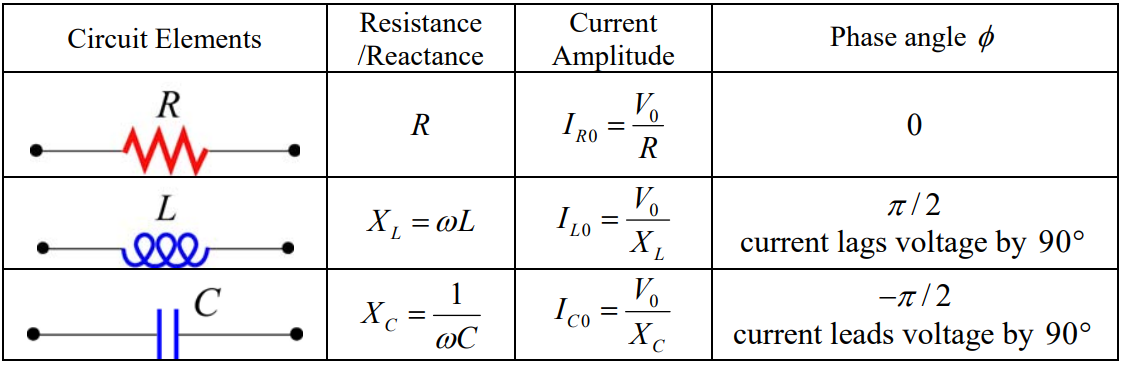
\includegraphics[width=0.8\textwidth]{ac1.PNG}
\end{center}
où $ X_L $ est la \textbf{réactance inductive} et $ X_C $ est la \textbf{réactance capacitive}.
    \item Pour les circuits qui ont plus d'un élément connectés en série, les résultats sont: 
\begin{center}
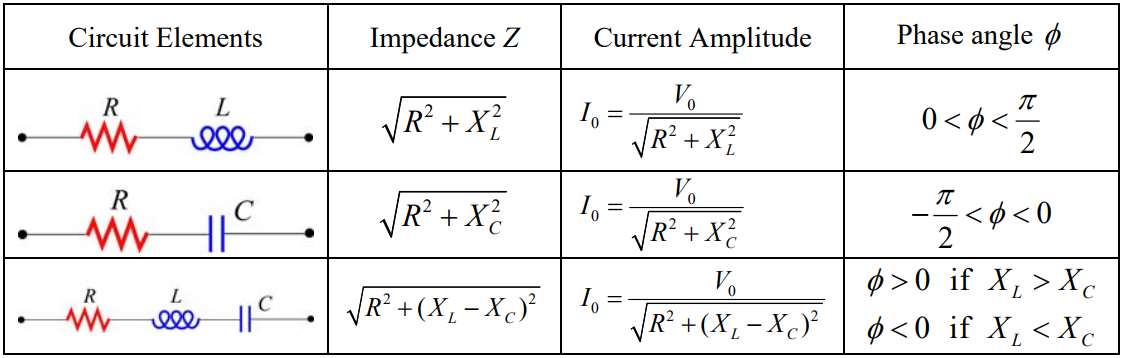
\includegraphics[width=0.8\textwidth]{ac2.PNG}
\end{center}
où $ Z $ est l'\textbf{impédance} $ Z $ du circuit. Pour un circuit RLC série, on a: 
\[ Z = \sqrt{R^2 + (X_L - X_C)^2} \]
L'angle de phase entre la tension (voltage) et le courant dans un circuit AC est: 
\[ \phi = \tan^{-1} \Big( \frac{X_L - X_C}{R} \Big) \]
    \item Dans un circuit RLC parallèle, l'impédance est donnée par:
\[ \frac{1}{Z} = \sqrt{ \frac{1}{R^2} + \Big( \omega C - \frac{1}{\omega L} \Big)^2 } = \sqrt{ \frac{1}{R^2} + \Big( \frac{1}{X_C} - \frac{1}{X_L} \Big)^2 } \]
et le déphasage est: 
\[ \phi = \tan^{-1} \Big[ R \Big( \frac{1}{X_C} - \frac{1}{X_L} \Big) \Big] = \tan^{-1} \Big[ R \Big( \omega C - \frac{1}{\omega L} \Big) \Big] \]
    \item Le voltage \textbf{rms} (root mean square = moyenne quadratique ; voltage rms = tension efficace) et la valeur efficace moyenne
du courant d'un circuit AC (AC = courant alternatif) sont données par: 
\[ V_{\text{eff}} = \frac{V_0}{\sqrt{2}}, \qquad I_{\text{eff}} = \frac{I_0}{\sqrt{2}} \]
    \item La puissance moyenne d'un circuit AC est: 
\[ \langle P(t) \rangle = I_{\text{eff}} V_{\text{eff}} \cos \phi \]
où $ \cos \phi $ est connu comme le \textbf{facteur de puissance}.
    \item La \textbf{fréquence de résonance} $ \omega_0 $ est: \[ \omega_0 = \frac{1}{\sqrt{LC}} \]
En \textbf{résonance}, le courant dans un circuit RLC série atteint son maximum, alors que le courant dans un circuit RLC parallèle atteint son minimum.
    \item L'équation du transformateur est: \[ \frac{V_2}{V_1} = \frac{N_2}{N_1} \]
où $ V_1 $ est la source de tension de la première bobine à $ N_1 $ boucles et $ V_2 $ est la tension de sortie (output voltage) de la seconde bobine à $ N_2 $ boucles. Un transformateur avec $ N_2 > N_1 $ est appelé transformateur élévateur (step-up transformer) et un transformateur avec $ N_2 < N_1 $ est appelé transformateur descendeur (step-down transformer).
\end{itemize}












\subsection{Aide pour la pratique}







Dans la sous-section "Théorie", on a vu comment les phaseurs peuvent fournir un outil puissant pour l'analyse des circuits AC \Big(En physique et en ingénierie, un phaseur est une représentation d'une fonction sinusoïdale dans laquelle l'amplitude $ A $, la phase $ \theta $ et la pulsation $ \omega $ (sachant que $ \omega = 2 \pi f $) ne dépendent pas du temps. Il s'agit d'une application d'un concept plus général appelé représentation analytique.\footnote{Wikipédia}\Big). Voici quelques conseils importants: 
\begin{enumerate}
    \item Garder à l'esprit les relations de phase pour les circuits les plus simples.
        \begin{enumerate}[i.]
            \item Pour une résistance, la tension (voltage) et le déphasage sont toujours en phase.
            \item Pour un inducteur, le courant a un retard de 90 ° sur la tension.
            \item Pour un condensateur, le courant est en avance de 90 ° sur la tension.
        \end{enumerate}
    \item Lorsque des éléments du circuits sont connectés en série, le courant instantané est le même pour tous les composants, et les
tensions instantanées à travers les éléments sont tous en phase. D'autre part, lorsque les éléments du circuit sont connectés en parallèle, la tension instantanée est la même pour tous les éléments, et les courants instantanés à travers les éléments ne sont pas en phase.
    \item Pour les connections en série, dessiner un diagramme de phase pour les tensions. Ici, un diagramme de phase d'un circuit RLC 
série est montré dans le cas inductif $ X_L > X_C $ et dans le cas capacitif $ X_L < X_C $.
\begin{center}
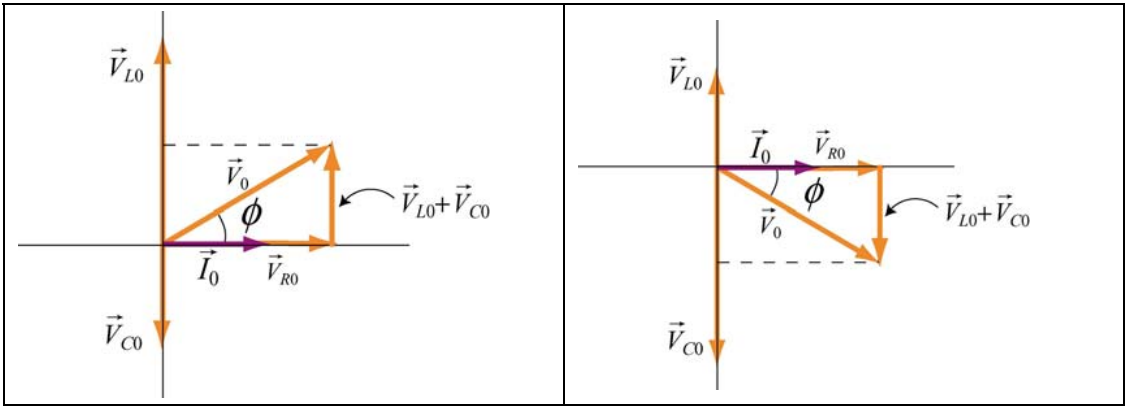
\includegraphics[width=0.8\textwidth]{ac3.PNG}
\end{center}
    \item Lorsque $ V_{L_0} = V_{C_0} $, ou $ \phi = 0 $, le circuit est en résonance. La fréquence de résonance correspondante est 
$\displaystyle \omega_0 = \frac{1}{\sqrt{LC}} $ et la puissance délivrée à la résistance est maximum.
    \item Pour les connections en parallèle, dessiner un diagramme de phase pour les courants. Ici, un diagramme de phase d'un circuit 
RLC parallèle est montré dans le cas inductif $ X_L > X_C $ et dans le cas capacitif $ X_L < X_C $.
\begin{center}
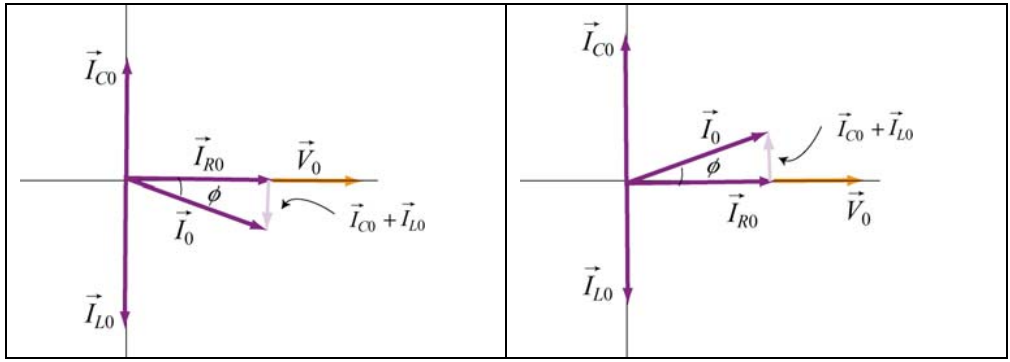
\includegraphics[width=0.8\textwidth]{ac4.PNG}
\end{center}
\end{enumerate}

























\section{Équations de Maxwell et ondes électromagnétiques}














\subsection{Théorie}








\begin{itemize}
    \item La \textbf{loi d'Ampère-Maxwell} dit que: 
\[ \oint \vec{\textbf{B}} \cdot d \vec{\textbf{s}} = \mu_0 I + \mu_0 \epsilon_0 \frac{d \Phi_E}{d t} = \mu_0 (I + I_d) \]
où $\displaystyle I_d = \epsilon_0 \frac{d \Phi_E}{d t} $ est appelé le \textbf{courant de déplacement}. L'équation décrit comment un flux électrique changeant peut induire un champ magnétique.
    \item La loi de Gauss pour le magnétisme est: 
\[ \Phi_B = \oiint_S \vec{\textbf{B}} \cdot d \vec{\textbf{A}} = 0 \]
La loi déclare que le flux magnétique traversant une surface fermée doit être égal à zéro, et implique l'absence de mono-pôles magnétiques.
    \item Tout phénomène électromagnétique est décrit par les \textbf{équations de Maxwell}: 
\begin{align*}
\oiint_S \vec{\textbf{E}} \cdot d \vec{\textbf{A}} &= \frac{Q}{\epsilon_0}  & \oint \vec{\textbf{E}} \cdot d \vec{\textbf{s}} &= - \frac{d \Phi_B}{d t} \\
\oiint_S \vec{\textbf{B}} \cdot d \vec{\textbf{A}} &= 0                     & \oint \vec{\textbf{B}} \cdot d \vec{\textbf{s}} &= \mu_0 I + \mu_0 \epsilon_0 \frac{d \Phi_E}{d t}
\end{align*}
    \item Dans le vide, les composantes électriques et magnétiques d'une onde électromagnétique obéissent à l'équation d'onde: 
\[ \bigg( \frac{\partial^2}{\partial x^2} - \mu_0 \epsilon_0 \frac{\partial^2}{\partial t^2} \bigg)
\begin{Bmatrix}
E_y (x, t) \\
B_z (x, t)
\end{Bmatrix} = 0 \]
    \item L'amplitude du champ électrique et du champ magnétique sont liées par: 
\[ \frac{E}{B} = \frac{E_0}{B_0} = \frac{\omega}{k} = c = \frac{1}{\sqrt{\mu_0 \epsilon_0}} = 3 \times 10^8 m / s \]
    \item Une \textbf{onde électromagnétique stationnaire} ne se propage pas, mais les champs électrique et magnétique exécutent des 
mouvements harmoniques simples perpendiculaire à la direction de propagation (si elle se propageait). Un exemple d'onde stationnaire est: 
\[ E_y(x, t) = 2 E_0 \sin k x \sin \omega t, \qquad B_z(x, t) = 2 B_0 \cos k x \cos \omega t \]
    \item Le débit d'énergie d'une onde électromagnétique traversant une surface fermée est donné par: 
\[ \frac{d U}{d t} = - \oiint \vec{\textbf{S}} \cdot d \vec{\textbf{A}} \]
où \[ \vec{\textbf{S}} = \frac{1}{\mu_0} \vec{\textbf{E}} \wedge \vec{\textbf{B}} \]
est le \textbf{vecteur de Poynting}, et $ \vec{\textbf{S}} $ pointe dans la direction vers laquelle l'onde se propage.
    \item L'\textbf{intensité} d'une onde électromagnétique est reliée à la densité moyenne d'énergie par: 
\[ I = \langle S \rangle = c \langle u \rangle \]
    \item Le moment de force transféré est relié à l'énergie absorbée par: 
\[ \Delta p = 
\begin{cases} \displaystyle
\frac{\Delta U}{c}      & \text{ (absorption totale) } \\ \\ \displaystyle
2 \frac{\Delta U}{c}    & \text{ (réflection totale) }
\end{cases} \]
    \item La \textbf{pression de rayonnement} moyenne sur une surface par une onde électromagnétique qui se dirige perpendiculairement 
vers cette surface est: 
\[ P = 
\begin{cases} \displaystyle
\frac{I}{c}             & \text{ (absorption totale) } \\ \\ \displaystyle
2 \frac{I}{c}           & \text{ (réflection totale) }
\end{cases} \]
\end{itemize}















\subsection{Pratique}








La sous-section "Théorie" explore diverses propriétés des ondes électromagnétiques. Les champs électrique et magnétique de l'onde obéissent à l'équation d'onde. Une fois que la forme fonctionnelle de l'un des champs est donnée, l'autre peut être déterminée à partir des équations de Maxwell. Par exemple, considérons une onde électromagnétique sinusoïdale avec: 
\[ \vec{\textbf{E}} (z, t) = E_0 \sin (k z - \omega t) \hat{\textbf{i}} \]
L'équation ci-dessus contient l'information complète sur l'onde électromagnétique: 
\begin{enumerate}
    \item Le sens de la propagation de l'onde: l'argument de la forme sinusoïdale dans le champ électrique peut être réécrit comme 
$ (k z - \omega t) = k (z - v t) $, ce qui indique que l'onde se propage dans la direction $ + z $.
    \item La longueur d'onde: la longueur d'onde $ \lambda $ est relié au nombre d'onde $ k $ par 
$\displaystyle \lambda = \frac{2 \pi}{k} $.
    \item La fréquence: la fréquence de l'onde $ f $ est liée à la fréquence angulaire $ \omega $ par 
$\displaystyle f = \frac{\omega}{2 \pi} $.
    \item La vitesse de propagation: la vitesse de l'onde est donnée par: 
\[ v = \lambda f = \frac{2 \pi}{k} \frac{\omega}{2 \pi} = \frac{\omega}{k} \]
Dans le vide, la vitesse de propagation d'une onde électromagnétique est égale à la vitesse de la lumière $ c $.
    \item Le champ magnétique $ \vec{\textbf{B}} $: le champ magnétique $ \vec{\textbf{B}} $ est perpendiculaire à la fois à 
$ \vec{\textbf{E}} $ qui pointe dans la direction $ + x $ et à $ + \hat{\textbf{k}} $, le vecteur unité le long de l'axe $ + z $ ; $ \hat{\textbf{k}} $ étant la direction de propagation de l'onde comme trouvé précédemment. De plus, puisque l'onde se propage dans la même direction que le produit vectoriel $ \vec{\textbf{E}} \wedge \vec{\textbf{B}} $, on en conclu que $ \vec{\textbf{B}} $ doit pointer dans la direction $ + y $ (étant donné que $ \hat{\textbf{i}} \wedge \hat{\textbf{j}} = \hat{\textbf{k}} $).

Comme $ \vec{\textbf{B}} $ est toujours en phase avec $ \vec{\textbf{E}} $, les deux champs ont la même forme fonctionnelle (same functional form). Et donc, on peut écrire le champ magnétique: 
\[ \vec{\textbf{B}} (z, t) = B_0 \sin (k z - \omega t) \hat{\textbf{j}} \]
où $ B_0 $ est l'amplitude. En utilisant les équations de Maxwell, il est possible de montrer que \\
$\displaystyle B_0 = E_0 \frac{k}{\omega} = \frac{E_0}{c} $ dans le vide.
    \item Le vecteur de Poynting: le vecteur de Poynting peut être obtenu ainsi: 
\[ \vec{\textbf{S}} = \frac{1}{\mu_0} \vec{\textbf{E}} \wedge \vec{\textbf{B}} = \frac{1}{\mu_0} \Big[ E_0 \sin (k z - \omega t) \hat{\textbf{i}} \Big] \wedge \Big[ B_0 \sin (k z - \omega t) \hat{\textbf{j}} \Big] = \frac{E_0 B_0 \sin^2 (k z - \omega t)}{\mu_0} \hat{\textbf{\textbf{k}}} \]
    \item L'intensité: L'intensité de l'onde est égale à la moyenne de $ S $: 
\[ I = \langle S \rangle = \frac{E_0 B_0}{\mu_0} \langle \sin^2 (k z - \omega t) \rangle = \frac{E_0 B_0}{2 \mu_0} = 
\frac{E_0^2}{2 c \mu_0} = \frac{c B_0^2}{2 \mu_0} \]
    \item La pression de radiation (électromagnétique): si l'onde électromagnétique se dirige perpendiculairement vers une surface et 
que le rayonnement (électromagnétique) est totalement \emph{réfléchi}, la pression de radiation vaut: 
\[ P = \frac{2 I}{c} = \frac{E_0 B_0}{c \mu_0} = \frac{E_0^2}{c^2 \mu_0} = \frac{B_0^2}{\mu_0} \]

\end{enumerate}






















\section{Interférence et diffraction}









\subsection{Théorie}







\begin{itemize}
    \item L'\textbf{interférence} est la combinaison de deux ou plusieurs ondes pour former une onde composite basée sur le principe de
la superposition.
    \item Dans l'\textbf{expérience à deux fentes de Young}, où une source de lumière monochromatique cohérente avec une longueur d'onde 
$ \lambda $ émerge de deux fentes qui sont séparées par une distance $ d $, la condition d'\textbf{interférence constructive} est: 
\[ \delta = d \sin \theta = m \lambda, \quad m = 0, \pm 1, \pm 2, \pm 3, ... \quad \text{ (interférence constructive) } \]
où $ m $ est appelé le numéro de commande (order number). D'autre part, la condition d'interférence destructrice est: 
\[ d \sin \theta = \Big( m + \frac{1}{2} \Big) \lambda, \quad m = 0, \pm 1, \pm 2, \pm 3, ... \quad \text{ (interférence destructive) } \]
    \item L' \textbf{intensité} dans le schéma d'interférence est: 
\[ I = I_0 \cos^2 \Big( \frac{\pi d \sin \theta}{\lambda} \Big) \]
où $ I_0 $ est l'intensité maximum sur l'écran.
    \item La \textbf{diffraction} La diffraction est la flexion des ondes lorsqu'elles passent par un objet (un objet est sur leur 
passage) ou par une ouverture. Dans une diffraction Fraunhofer à une seule fente, la condition pour l'interférence destructrice est: 
\[ \sin \theta = m \frac{\lambda}{a}, \quad m = \pm 1, \pm 2, \pm 3, ... \quad \textbf{ (interférence destructive) } \]
où $ a $ est la largeur de la fente. L'intensité du modèle (pattern) d'interférence est: 
\[ I = I_0 \Big[ \frac{\sin (\beta / 2)}{\beta / 2} \Big]^2 = \Big[ \frac{\sin (\pi a \sin \theta / \lambda)}{\pi a \sin \theta / \lambda} \Big]^2 \]
où $ \beta = 2 \pi a \sin \theta / \lambda $ est la différence de déphasage totale entre les ondes de l'extrémité supérieure et de l'extrémité inférieure de la fente, et $ I_0 $ est l'intensité pour $ \theta = 0 $.
    \item Pour deux fentes ayant chacune une largeur $ a $ et séparées par une distance $ d $, le motif d'interférence inclura également 
un motif de diffraction dû à la fente unique, et l'intensité est: 
\[ I = I_0 \cos^2 \bigg( \frac{\pi d \sin \theta}{\lambda} \bigg) \bigg[ \frac{\sin (\pi a \sin \theta / \lambda)}{\pi a \sin \theta / \lambda} \bigg]^2 \]
\end{itemize}






















\section{Annexe}











\subsection{Démonstration: loi de Gauss}









\subsubsection{Rappel: stéradian}

\emph{Rappel}: 
\begin{center}
\begin{tabular}{p{7cm}|p{7cm}}
Cercle & Sphère \\
\hline
 & \\
Le cercle est à 2 dimensions. & La sphère est à 3 dimensions. \\
rayon = R, angle = $ \theta $ & rayon = R, angle solide (stéradian) = $ \Omega $ \\
Tout le cercle: $ L = 2 \pi R $ & Toute la sphère: $ A = 4 \pi R^2 $ \\
$ L = R \theta \qquad \theta \in [0, 2 \pi] $ & $ A = R^2 \Omega \qquad \Omega \in [0, 4 \pi] $ \\
 & \\
\centering 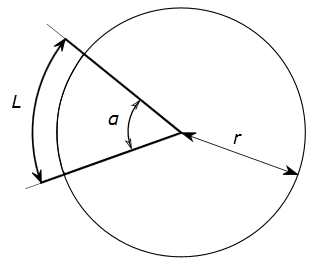
\includegraphics[width=0.20\textwidth]{cercle.png} & \centering 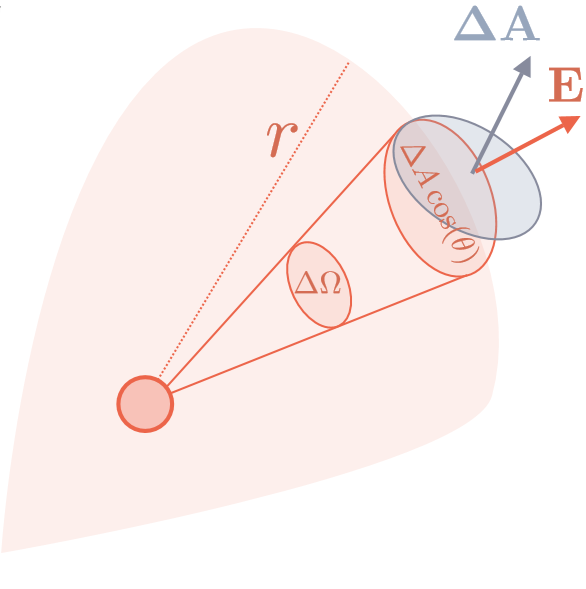
\includegraphics[width=0.20\textwidth]{steradian.PNG}
\end{tabular}
\end{center}









\subsubsection{Démonstration}







La \textbf{loi de Gauss} affirme que le flux électrique passant au travers de n'importe quelle surface de Gauss est 
proportionnel à la charge totale enfermée par cette surface: \[ \Phi_E = \oiint_S \vec{\textbf{E}} \cdot d \vec{\textbf{A}} = \frac{q}{\epsilon_0} \]

\newpage

On sait que: 
\begin{enumerate}
    \item $\displaystyle \Phi_E = \vec{\textbf{E}} \cdot \vec{\textbf{A}} $
    \item La charge est entourée par une surface $ A $ ($ A $ est une surface dans un espace à 3 dimensions).
\begin{center}
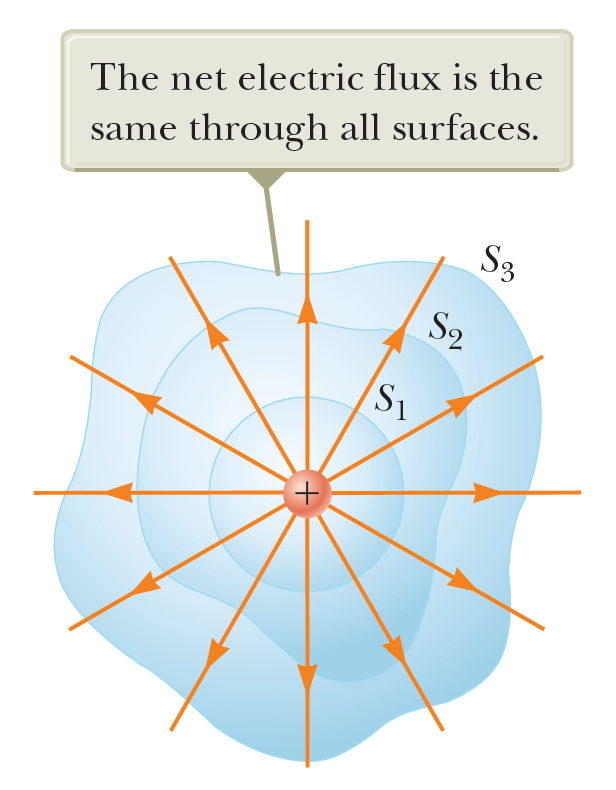
\includegraphics[width=0.35\textwidth]{FluxElectrique.PNG}
\end{center}
\end{enumerate}

Démonstration: \\
Le flux du champ électrique total 
\[
\Phi_E = \lim_{n \to \infty} \sum_{i = 1}^n \textbf{E} \cdot \Delta \textbf{A}_i = \lim_{n \to \infty} \sum_{i = 1}^{n} \Delta \Phi_i
\]

\[
\Delta \Phi_i = \textbf{E} \cdot \Delta \textbf{A}_i = E \cos(\theta) \Delta A_i = \frac{1}{4 \pi \epsilon_0} \frac{q}{r^2} \cos(\theta) \Delta A = \frac{1}{4 \pi \epsilon_0} q \Delta \Omega
\]

\[
\implies \Phi_E = \oint \frac{1}{4 \pi \epsilon_0} q d\Omega = \frac{q}{4 \pi \epsilon_0} 4 \pi = \frac{q}{\epsilon_0}
\]

\[ \boxed{ \Phi_E = \frac{q}{\epsilon_0} } \]
Le flux du champs électrique total est indépendant de la forme de la surface fermée et indépendant de la position de la charge dans le volume délimité par la surface. \\

\emph{Remarque (Importante)}: \\
Le théorème de Gauss dit que le flux est proportionnel à la charge pas le champs électrique.















\subsection{Combinaisons de composants électriques}







\subsubsection{Combinaisons de condensateurs}






\begin{center}

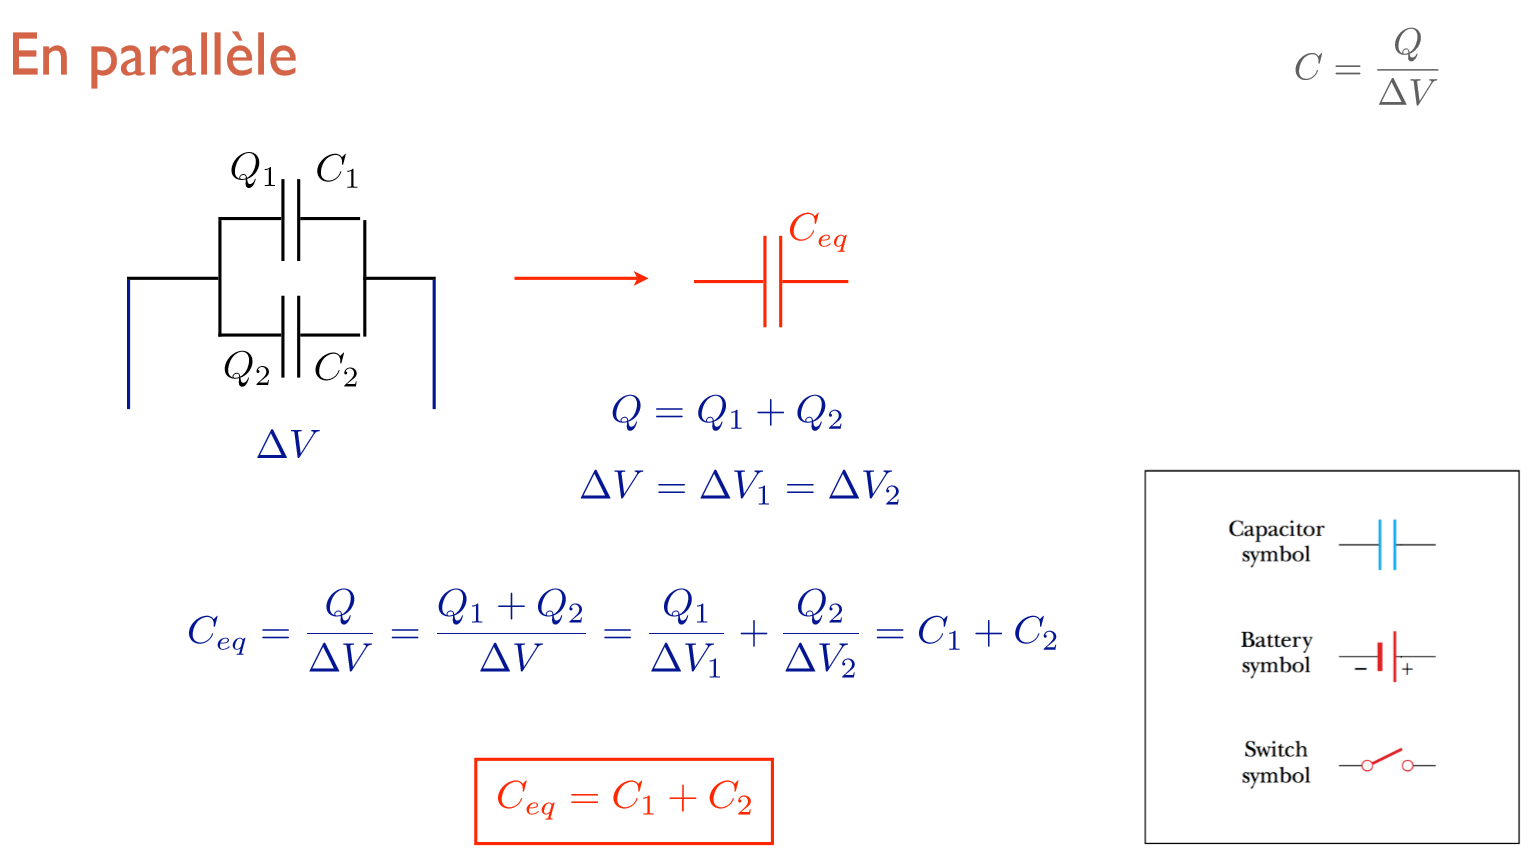
\includegraphics[width=\textwidth]{CondP.PNG}
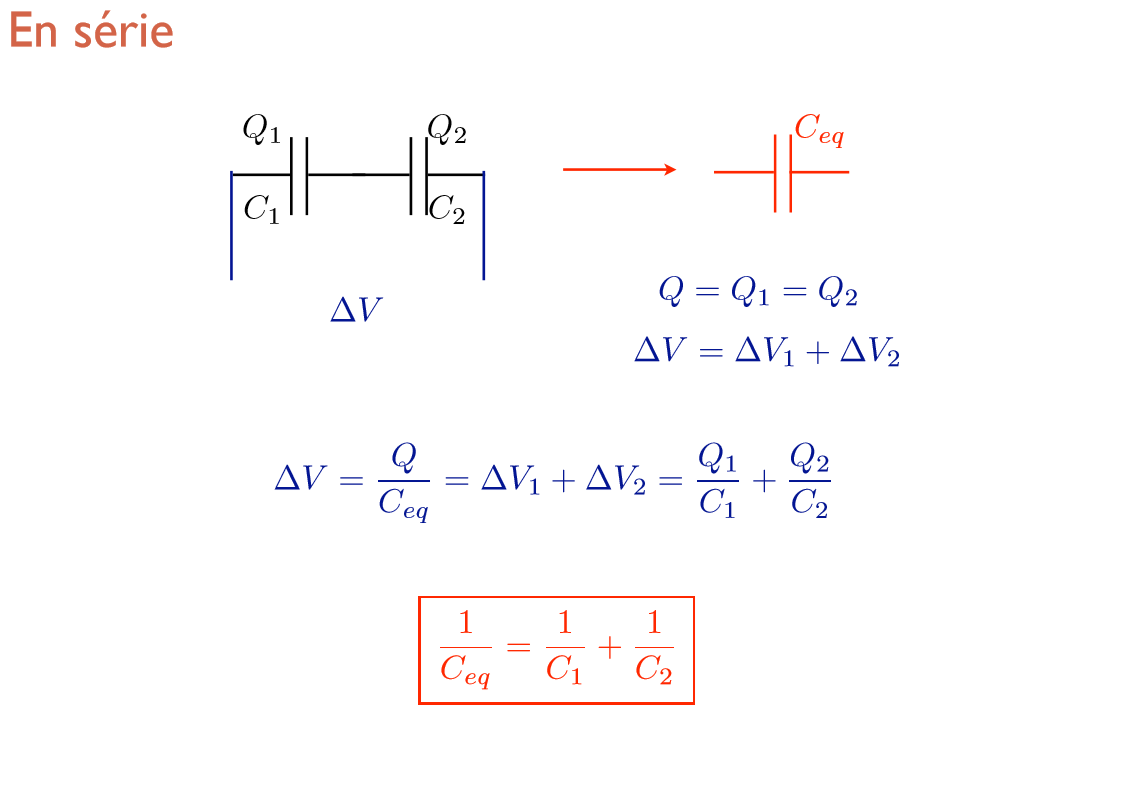
\includegraphics[width=\textwidth]{CondS.PNG}

\end{center}






\subsubsection{Association de piles}





\begin{center}

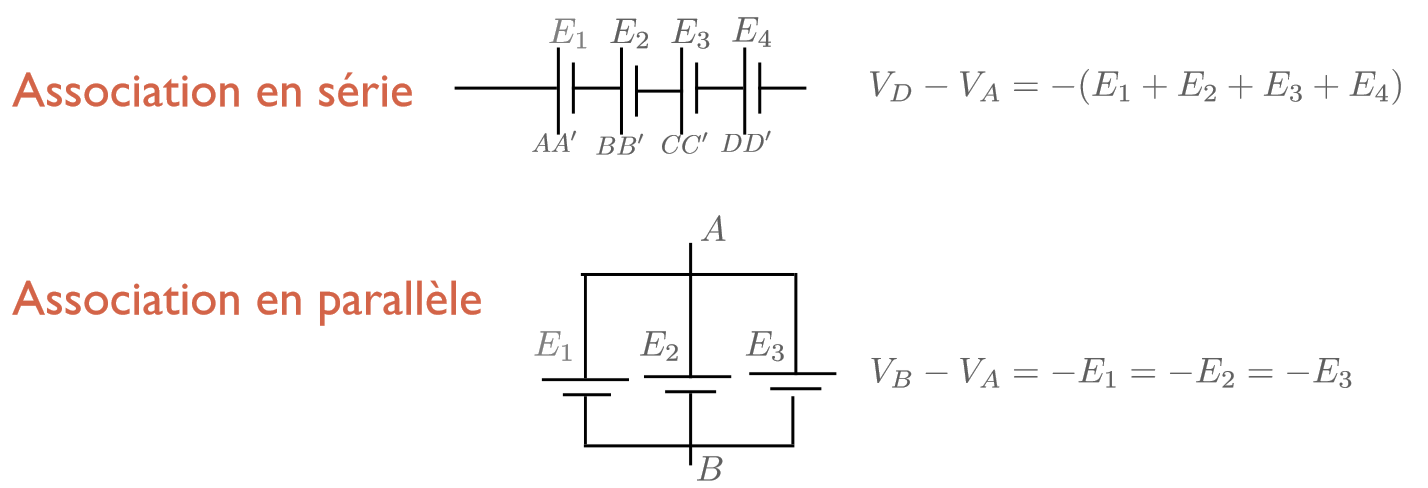
\includegraphics[width=\textwidth]{AssosPiles.PNG}

\end{center}






\subsubsection{Association de résistance}





\begin{center}

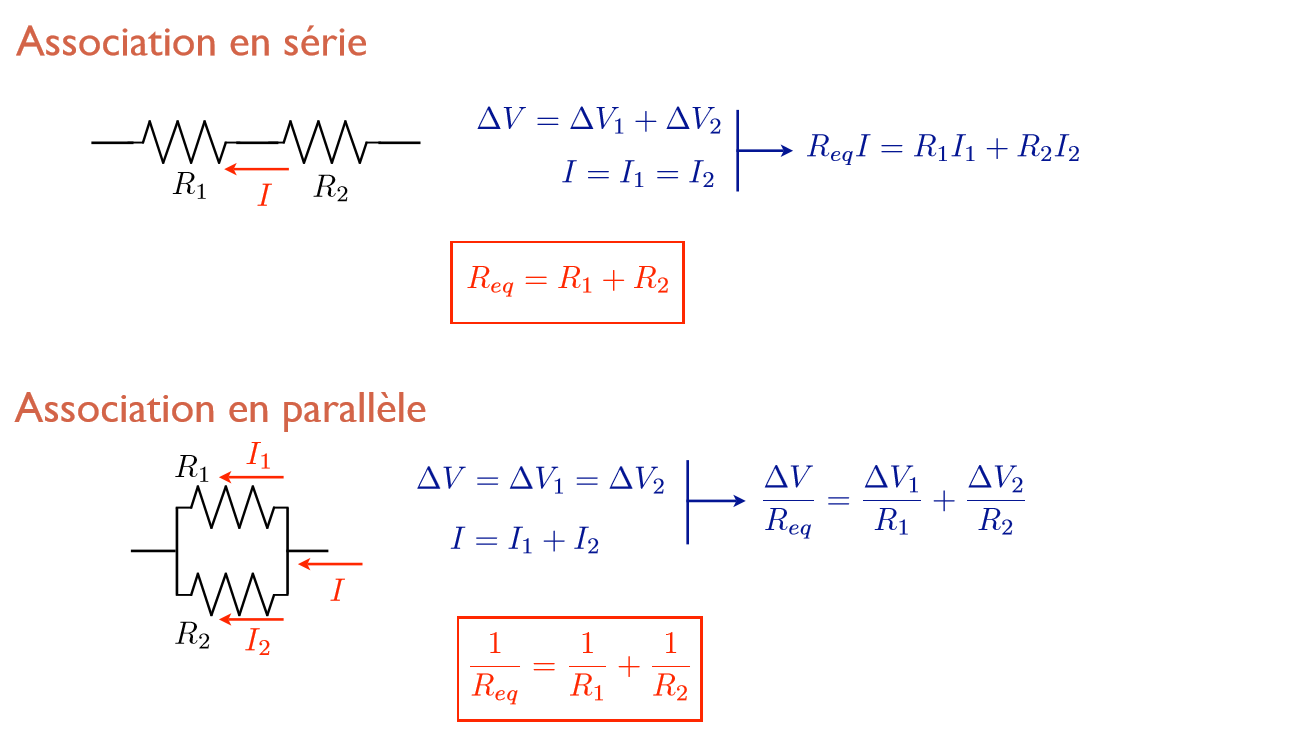
\includegraphics[width=\textwidth]{AssosResist.PNG}

\end{center}






































\end{document}
